\documentclass[12pt,a4paper]{report}
\usepackage{fontspec}
\IfFontExistsTF{Times New Roman}{\setmainfont{Times New Roman}}{\IfFontExistsTF{TeX Gyre Termes}{\setmainfont{TeX Gyre Termes}}{\setmainfont{Liberation Serif}}}
\usepackage{polyglossia}
\setdefaultlanguage{vietnamese}
\usepackage[a4paper,left=3cm,right=2cm,top=2.5cm,bottom=2.5cm]{geometry}
\usepackage{setspace}
\usepackage{graphicx}
\usepackage{pdfpages}
\setkeys{Gin}{draft=false}
\usepackage{float}
\usepackage{booktabs}
\usepackage{longtable}
\usepackage{tabularx}
\usepackage{makecell}
\usepackage{array}
\usepackage{ragged2e}
\usepackage{multirow}
\usepackage{xcolor}
\usepackage{caption}
\usepackage{subcaption}
\usepackage{amsmath}
\usepackage{amssymb}
\usepackage{tikz}
\usetikzlibrary{arrows.meta,positioning,shapes.geometric}
\usepackage{listings}
\lstdefinelanguage{json}{
    basicstyle=\ttfamily\small,
    showstringspaces=false,
    breaklines=true,
    frame=single,
    columns=fullflexible,
    morestring=[b]",
    stringstyle=\color{black},
    literate=
     *{0}{{{0}}}{1}{1}{{{1}}}{1}{2}{{{2}}}{1}{3}{{{3}}}{1}{4}{{{4}}}{1}
      {5}{{{5}}}{1}{6}{{{6}}}{1}{7}{{{7}}}{1}{8}{{{8}}}{1}{9}{{{9}}}{1}
}

\usepackage{enumitem}
\usepackage[protrusion=true,expansion=false]{microtype}
\usepackage{xurl}
\usepackage{url}
\usepackage{seqsplit}
\usepackage{hyperref}
\hypersetup{hidelinks}
\pdfstringdefDisableCommands{%
  \def\TFIDF{TF-IDF}%
  \def\MacroFOne{macro-F1}%
  \def\EvidenceGrounded{evidence-grounded}%
  \def\MultilingualE{multilingual-E5}%
  \def\RatingSentiment{rating-sentiment}%
  \def\HumanInLoop{human-in-the-loop}%
}

\Urlmuskip=0mu plus 2mu
\AtBeginDocument{\fontsize{13pt}{19.5pt}\selectfont}
\onehalfspacing
\setlength{\parindent}{0pt}
\setlength{\parskip}{0.75em}
\renewcommand{\arraystretch}{1.25}
\setlist[itemize]{leftmargin=1.2cm}
\setlist[enumerate]{leftmargin=1.2cm}
\DeclareRobustCommand{\code}[1]{\path{#1}}
\DeclareRobustCommand{\codepath}[1]{\path{#1}}
\DeclareRobustCommand{\filepath}[1]{\path{#1}}
% Macros for frequent technical terms. They prevent awkward line breaks in the PDF.
\DeclareRobustCommand{\TFIDF}{\texorpdfstring{\mbox{TF-IDF}}{TF-IDF}}
\DeclareRobustCommand{\MacroFOne}{\texorpdfstring{\mbox{macro-F1}}{macro-F1}}
\DeclareRobustCommand{\EvidenceGrounded}{\texorpdfstring{\mbox{evidence-grounded}}{evidence-grounded}}
\DeclareRobustCommand{\MultilingualE}{\texorpdfstring{\mbox{multilingual-E5}}{multilingual-E5}}
\DeclareRobustCommand{\RatingSentiment}{\texorpdfstring{\mbox{rating-sentiment}}{rating-sentiment}}
\DeclareRobustCommand{\HumanInLoop}{\texorpdfstring{\mbox{human-in-the-loop}}{human-in-the-loop}}

\newcolumntype{L}[1]{>{\RaggedRight\arraybackslash}p{#1}}
\newcolumntype{Y}{>{\RaggedRight\arraybackslash}X}
\newcommand{\studentNameValue}{Họ tên sinh viên}
\newcommand{\studentIdValue}{MSSV}
\newcommand{\universityNameValue}{Tên trường}
\newcommand{\facultyNameValue}{Tên khoa/bộ môn}
\newcommand{\instructorNameValue}{Tên giảng viên}
\newcommand{\reportDateValue}{Tháng/Năm}
\newcommand{\studentName}[1]{\renewcommand{\studentNameValue}{#1}}
\newcommand{\studentId}[1]{\renewcommand{\studentIdValue}{#1}}
\newcommand{\universityName}[1]{\renewcommand{\universityNameValue}{#1}}
\newcommand{\facultyName}[1]{\renewcommand{\facultyNameValue}{#1}}
\newcommand{\instructorName}[1]{\renewcommand{\instructorNameValue}{#1}}
\newcommand{\reportDate}[1]{\renewcommand{\reportDateValue}{#1}}
% ===== THÔNG TIN TRANG BÌA - sửa các dòng dưới đây trước khi nộp =====
\studentName{\begin{tabular}[t]{@{}l@{}}Tạ Chí Bình -- 2351060002\\Phan Tấn Phúc -- 2351060029\\Phạm Nguyễn Bảo Vi -- 2351060041\end{tabular}}
\studentId{}
\universityName{Trường Đại học Mở Thành phố Hồ Chí Minh}
\facultyName{Khoa Khoa học Cơ bản}
\instructorName{Hà Minh Tuấn}
\reportDate{TP.HCM, tháng 05 năm 2026}
\emergencystretch=4em
\tolerance=2000
\hbadness=10000
\renewcommand{\contentsname}{Mục lục}
\renewcommand{\listfigurename}{Danh mục hình}
\renewcommand{\listtablename}{Danh mục bảng}
% Mục lục gọn theo phong cách bài báo/arXiv: hiện chương và mục chính, ẩn tiểu mục quá chi tiết.
\setcounter{tocdepth}{1}
\setcounter{secnumdepth}{3}

\newcommand{\safeimage}[4]{%
\IfFileExists{#1}{%
\begin{figure}[H]
    \centering
    \includegraphics[width=#4]{#1}
    \caption{#2}
    \label{#3}
\end{figure}
}{}%
}

\newcommand{\optionalimage}[4]{%
\IfFileExists{#1}{%
\begin{figure}[H]
    \centering
    \includegraphics[width=#4]{#1}
    \caption{#2}
    \label{#3}
\end{figure}
}{}%
}
\lstset{basicstyle=\ttfamily\small,breaklines=true,frame=single,columns=fullflexible,keepspaces=true,showstringspaces=false,backgroundcolor=\color{gray!5}}
\newenvironment{keepcode}{\par\noindent\begin{minipage}{\textwidth}}{\end{minipage}\par}
\begin{document}
\pagenumbering{gobble}

\includepdf[pages=1-3,pagecommand={},width=\paperwidth]{cover_nlp.pdf}
\chapter*{Tóm tắt tiếng Việt}
Đề tài xây dựng một hệ thống xử lý review thương mại điện tử tiếng Việt theo hai hướng chính. Thứ nhất, hệ thống huấn luyện mô hình phân loại cảm xúc review thành ba lớp: tiêu cực, trung lập và tích cực. Các mô hình baseline gồm majority baseline, \TFIDF{} kết hợp Logistic Regression và \TFIDF{} kết hợp Linear SVM. Kết quả thực nghiệm cho thấy Linear SVM là mô hình tốt nhất trong các baseline đã thử, đạt test accuracy khoảng 0,9329 và test \MacroFOne{} khoảng 0,9098. Thứ hai, hệ thống xây dựng tầng Retrieval-Augmented Generation dạng \EvidenceGrounded{}: người dùng đặt câu hỏi về review, hệ thống truy xuất các review liên quan từ FAISS index, sau đó tạo câu trả lời theo template có citation. Bản final dùng 82.677 documents, embedding model \code{intfloat/multilingual-e5-small}, vector dim 384 và FAISS \code{IndexFlatIP}. Đề tài cũng bổ sung Module 6 như một hướng nâng cấp retrieval bằng BM25, Dense FAISS, RRF fusion, reranking nhẹ và rule-based aspect analysis. Hệ thống có giao diện thử nghiệm gồm ba tab: phân tích sentiment, hỏi đáp RAG và kỹ thuật/đánh giá.
\cleardoublepage
\tableofcontents
\cleardoublepage
\renewcommand{\listfigurename}{Danh mục hình}
\listoffigures
\cleardoublepage
\renewcommand{\listtablename}{Danh mục bảng}
\listoftables
\cleardoublepage
\chapter*{Danh mục từ viết tắt}
\begin{longtable}{p{0.22\textwidth}p{0.68\textwidth}}
\toprule
Từ viết tắt & Ý nghĩa \\
\midrule
NLP & Natural Language Processing, xử lý ngôn ngữ tự nhiên. \\
TMĐT & Thương mại điện tử. \\
RAG & Retrieval-Augmented Generation, tạo câu trả lời có hỗ trợ bởi truy xuất tài liệu. \\
\TFIDF{} & Term Frequency--Inverse Document Frequency. \\
SVM & Support Vector Machine. \\
FAISS & Facebook AI Similarity Search. \\
BM25 & Hàm xếp hạng truy xuất dựa trên từ khóa. \\
RRF & Reciprocal Rank Fusion. \\
ABSA & Aspect-Based Sentiment Analysis. \\
\bottomrule
\end{longtable}
\cleardoublepage
\pagenumbering{arabic}
\chapter{Mở đầu}
\section{Bối cảnh thương mại điện tử và dữ liệu review}
Thương mại điện tử tạo ra một lượng lớn dữ liệu đánh giá sản phẩm mỗi ngày. Mỗi review có thể chứa thông tin về chất lượng sản phẩm, tốc độ giao hàng, đóng gói, phản hồi của shop, sai mẫu, thiếu hàng, kích thước, giá cả hoặc trải nghiệm sau bán. Với người mua, review giúp ra quyết định mua hàng. Với người bán, review là nguồn tín hiệu để phát hiện vấn đề vận hành. Với nền tảng TMĐT, review là dữ liệu quan trọng để đánh giá chất lượng nhà bán, sản phẩm và dịch vụ logistics.

Tuy nhiên, khi số lượng review lớn, việc đọc thủ công trở nên không khả thi. Một sản phẩm hoặc một ngành hàng có thể có hàng nghìn review. Người quản lý không chỉ muốn biết review là tích cực hay tiêu cực, mà còn muốn hỏi các câu như: khách hàng phàn nàn gì về giao hàng chậm, review nào nói shop giao thiếu hàng, hay vấn đề chất lượng sản phẩm xuất hiện ở đâu. Những câu hỏi này đòi hỏi hệ thống vừa biết phân tích cảm xúc vừa biết truy xuất bằng chứng cụ thể.

Trong bối cảnh đó, NLP giúp tự động hóa việc hiểu văn bản review, còn retrieval và RAG giúp tìm đúng các review làm bằng chứng. Điểm quan trọng của đề tài không phải chỉ là tạo một câu trả lời nghe có vẻ đúng, mà là tạo câu trả lời có thể kiểm chứng bằng review thật. Vì vậy hệ thống đặt trọng tâm vào evidence, citation và các metric thực nghiệm.

\section{Vấn đề cần giải quyết}
Đề tài tập trung vào hai vấn đề. Vấn đề thứ nhất là phân loại cảm xúc review tiếng Việt thành ba lớp: negative, neutral và positive. Đây là bài toán text classification điển hình trong NLP. Input là nội dung review; output là nhãn sentiment. Vấn đề thứ hai là hỏi đáp dựa trên review: khi người dùng đặt câu hỏi, hệ thống cần tìm các review liên quan và tạo câu trả lời có trích dẫn. Đây là hướng Retrieval-Augmented Generation, nhưng trong phạm vi đề tài này phần generation được thiết kế theo template và chỉ dựa trên evidence, không gọi API LLM bên ngoài.

Cách tiếp cận này phù hợp với yêu cầu học thuật vì kết quả có thể kiểm chứng. Nếu hệ thống nói khách hàng phàn nàn về giao hàng, báo cáo phải chỉ ra review nào là bằng chứng. Điều này khác với việc chỉ sinh câu trả lời tự do mà không có nguồn.

\section{Lý do chọn đề tài}
Đề tài được chọn vì kết hợp được nhiều kiến thức cốt lõi của môn NLP: tiền xử lý văn bản, biểu diễn văn bản, phân loại văn bản, đánh giá mô hình, embedding, retrieval, RAG và thiết kế giao diện thử nghiệm. Bên cạnh đó, dữ liệu review TMĐT gần gũi với thực tế và có tính ứng dụng cao. Hệ thống có thể hỗ trợ người bán tổng hợp phản hồi khách hàng, giúp người mua tìm hiểu vấn đề thường gặp, hoặc giúp nhóm vận hành phát hiện lỗi dịch vụ.

\section{Mục tiêu nghiên cứu}
Các mục tiêu chính của đề tài gồm:
\begin{itemize}
    \item Xây dựng pipeline dữ liệu cho review tiếng Việt, gồm làm sạch, xử lý duplicate, ánh xạ rating sang sentiment và chia train/valid/test.
    \item Huấn luyện và đánh giá các mô hình sentiment classification baseline, gồm majority baseline, TF-IDF + Logistic Regression và TF-IDF + Linear SVM.
    \item Xây dựng RAG corpus, embedding review bằng multilingual-E5, lưu FAISS index và metadata phục vụ retrieval.
    \item Tạo câu trả lời RAG có cấu trúc gồm tóm tắt, vấn đề chính, bằng chứng và độ tin cậy.
    \item Xây dựng giao diện thử nghiệm có ba tab: phân tích sentiment, hỏi đáp RAG và kỹ thuật/đánh giá.
    \item Bổ sung Module 6 như hướng nâng cấp retrieval bằng BM25, Dense FAISS, RRF fusion và aspect-aware reranking.
\end{itemize}

\section{Đối tượng và phạm vi nghiên cứu}
Đối tượng nghiên cứu là review sản phẩm TMĐT tiếng Việt. Phạm vi của đề tài là phân loại sentiment ở mức review và truy xuất bằng chứng review theo câu hỏi. Hệ thống không xây dựng chatbot LLM hoàn chỉnh, không huấn luyện mô hình ngôn ngữ lớn, và không khẳng định đã đạt mức production. Các kết quả retrieval được đánh giá ở mức baseline/manual evaluation, còn Module 6 là benchmark nhỏ mang tính chẩn đoán.

\section{Đóng góp chính}
Đóng góp của đề tài nằm ở tính end-to-end của pipeline. Module 2 tạo mô hình sentiment để phân loại review. Module 4 tạo tầng RAG có citation, giúp câu trả lời luôn gắn với review được truy xuất. Module 6 chỉ ra hướng cải thiện retrieval khi dense retrieval bỏ sót các cụm complaint ngắn. Tầng giao diện thử nghiệm minh họa cách vận hành của hệ thống qua ba thành phần tách biệt: dự đoán cảm xúc một review, hỏi đáp dựa trên nhiều review và hiển thị thông tin kỹ thuật/đánh giá.

\section{Cấu trúc báo cáo}
Báo cáo gồm mười một chương. Chương 1 trình bày bối cảnh và mục tiêu. Chương 2 trình bày cơ sở lý thuyết. Chương 3 mô tả yêu cầu và thiết kế hệ thống. Chương 4 trình bày dữ liệu và tiền xử lý. Chương 5 mô tả phương pháp theo từng module. Chương 6 trình bày thực nghiệm và kết quả. Chương 7 phân tích lỗi. Chương 8 mô tả triển khai thử nghiệm và giao diện hệ thống. Chương 9 thảo luận. Chương 10 nêu hạn chế và hướng phát triển. Chương 11 kết luận. Phụ lục trình bày cấu trúc thư mục, artifact, API, ví dụ input/output, pseudocode và bảng metric bổ sung.

\chapter{Cơ sở lý thuyết}
\section{Xử lý ngôn ngữ tự nhiên}
Xử lý ngôn ngữ tự nhiên, hay NLP, là lĩnh vực nghiên cứu cách máy tính xử lý, hiểu và sinh ngôn ngữ của con người \cite{jurafsky2023speech}. Trong đề tài này, NLP xuất hiện ở nhiều tầng: làm sạch review, biểu diễn văn bản bằng \TFIDF{}, phân loại sentiment, biểu diễn câu bằng embedding, truy xuất review liên quan và tạo câu trả lời dựa trên bằng chứng.

Văn bản tiếng Việt có một số đặc thù. Từ có thể gồm nhiều âm tiết cách nhau bằng khoảng trắng, ví dụ “giao hàng”, “chất lượng”, “không trả lời”. Người dùng thường viết tắt, thiếu dấu, dùng emoji hoặc lặp ký tự. Review TMĐT còn có nhiều câu rất ngắn như “ok”, “tạm được”, “giao lâu”, hoặc câu dài nhưng nhiễu do người dùng viết để nhận xu. Vì vậy tiền xử lý và lựa chọn mô hình cần chú ý đến nhiễu dữ liệu.

\section{Tiền xử lý văn bản}
Tiền xử lý văn bản là bước chuyển dữ liệu thô thành dạng có thể dùng cho mô hình. Với review TMĐT, các bước phổ biến gồm chuẩn hóa Unicode, loại bỏ HTML, xóa khoảng trắng thừa, kiểm tra giá trị rỗng, chuẩn hóa rating và xử lý duplicate. Trong đề tài, Module 1 thực hiện các bước này trước khi tạo tập train/valid/test cho sentiment và corpus cho RAG.

Tiền xử lý không nên làm mất thông tin quan trọng. Ví dụ, từ “không” là tín hiệu phủ định quan trọng; nếu xóa tùy tiện, câu “không tốt” có thể bị hiểu thành “tốt”. Các từ như “lỗi”, “chậm”, “thiếu”, “sai”, “hỏng”, “bể”, “vỡ”, “kém”, “tệ” cũng là tín hiệu complaint quan trọng cho retrieval.

\section{Phân tích cảm xúc}
Phân tích cảm xúc là bài toán xác định thái độ hoặc cảm xúc được thể hiện trong văn bản. Trong đề tài này, sentiment được chia thành ba lớp: negative, neutral và positive. Review “Shop giao sai màu, nhắn tin không trả lời” thường là negative. Review “Sản phẩm dùng ổn, giao nhanh” thường là positive. Review “Tạm được, chưa dùng lâu nên chưa biết” có thể là neutral.

Bài toán sentiment classification trong đề tài nhận input là một review và output là nhãn sentiment. Đây là bài toán phân loại văn bản có giám sát, vì dữ liệu train có nhãn. Nhãn được ánh xạ từ rating: 1--2 sao là negative, 3 sao là neutral, 4--5 sao là positive. Cách ánh xạ này đơn giản và phù hợp với dữ liệu có rating, nhưng có thể tạo nhiễu vì rating không luôn phản ánh đúng nội dung review.

\section{\TFIDF{}}
\TFIDF{} là phương pháp biểu diễn văn bản bằng vector dựa trên tần suất từ \cite{salton1988term}. TF đo một từ xuất hiện nhiều hay ít trong một văn bản. IDF giảm trọng số của các từ xuất hiện ở quá nhiều văn bản. Ví dụ, trong review TMĐT, từ “sản phẩm” có thể xuất hiện rất nhiều nên ít phân biệt. Ngược lại, các từ “giao sai”, “móp”, “không trả lời”, “hỏng” có thể mang nhiều thông tin hơn.

Với \TFIDF{}, câu “shop giao sai màu” được chuyển thành vector sparse, trong đó các chiều tương ứng với từ hoặc n-gram như “shop”, “giao”, “sai”, “màu”, “giao sai”. Hệ thống dùng n-gram 1--2 trong mô hình tốt nhất, tức là xét cả từ đơn và cụm hai từ. Điều này quan trọng vì cụm “không tốt” khác nhiều so với từ “tốt” đứng riêng.

\section{Logistic Regression và Linear SVM}
Logistic Regression là mô hình tuyến tính dùng để ước lượng xác suất một mẫu thuộc về từng lớp. Với text classification, input là vector \TFIDF{}, output là xác suất hoặc điểm cho các lớp negative, neutral, positive. Mô hình học trọng số cho từng từ/cụm từ. Nếu từ “tệ”, “lỗi”, “không trả lời” thường xuất hiện trong review negative, trọng số của chúng cho lớp negative sẽ lớn.

Linear SVM là mô hình phân loại tuyến tính tìm siêu phẳng phân tách các lớp với biên lớn \cite{cortes1995support}. Trong dữ liệu text, vector \TFIDF{} thường có số chiều lớn và sparse. Linear SVM phù hợp với dạng dữ liệu này vì nó hoạt động tốt trên không gian chiều cao và thường cho kết quả mạnh trong text classification \cite{fan2008liblinear}. Trong thực nghiệm của đề tài, Linear SVM đạt kết quả cao nhất trong các baseline đã thử: test accuracy khoảng 0,9329 và test \MacroFOne{} khoảng 0,9098.

\section{Majority baseline và các metric}
Majority baseline là mô hình rất đơn giản: luôn dự đoán lớp xuất hiện nhiều nhất trong tập train. Mô hình này không có giá trị ứng dụng cao, nhưng là mốc tối thiểu để so sánh. Nếu mô hình phức tạp không vượt được majority baseline, mô hình đó không hữu ích.

Accuracy là tỷ lệ dự đoán đúng trên toàn bộ mẫu. Precision của một lớp đo trong các mẫu được dự đoán là lớp đó, bao nhiêu mẫu thật sự đúng. Recall đo trong các mẫu thật sự thuộc lớp đó, mô hình tìm đúng được bao nhiêu. F1-score là trung bình điều hòa của precision và recall. Macro-F1 tính F1 trung bình đều cho từng lớp, không phụ thuộc lớp nhiều hay ít mẫu. Weighted-F1 cũng trung bình theo lớp nhưng có trọng số theo số mẫu. Trong dữ liệu lệch lớp, \MacroFOne{} quan trọng vì nó không để lớp lớn che khuất lớp nhỏ.


\section{Các công thức nền tảng}
Các metric và thuật toán trong báo cáo có thể tóm tắt bằng một số công thức chính. \TFIDF{} được viết ở dạng khái niệm:
\begin{equation}
\mathrm{tfidf}(t,d)=\mathrm{tf}(t,d)\times \log\frac{N}{\mathrm{df}(t)}.
\end{equation}
Công thức này làm nổi bật các từ/cụm từ phân biệt như "giao sai", "hàng lỗi", "không trả lời", đồng thời giảm trọng số từ quá phổ biến như "sản phẩm" \cite{salton1988term,manning2008ir}.

Với một lớp sentiment, precision, recall và F1 được tính như sau:
\begin{align}
\mathrm{Precision} &= \frac{TP}{TP+FP},\\
\mathrm{Recall} &= \frac{TP}{TP+FN},\\
F_1 &= \frac{2\times \mathrm{Precision}\times \mathrm{Recall}}{\mathrm{Precision}+\mathrm{Recall}}.
\end{align}
Macro-F1 tính trung bình đều theo lớp:
\begin{equation}
\mathrm{MacroF1}=\frac{1}{C}\sum_{c=1}^{C}F_{1,c}.
\end{equation}
Vì neutral chỉ chiếm 871/5.162 review sau dedup, \MacroFOne{} phù hợp hơn accuracy khi chọn mô hình.

Với embedding đã normalize, inner product tương đương cosine similarity:
\begin{equation}
\cos(q,d)=\frac{q\cdot d}{\|q\|\|d\|}=q\cdot d \quad \text{khi } \|q\|=\|d\|=1.
\end{equation}
Đây là lý do Module 4 dùng FAISS \code{IndexFlatIP} cho embedding \MultilingualE{} \cite{johnson2019billion,wang2022e5}.

Linear SVM tối ưu biên phân tách lớn. Ở mức khái niệm, binary SVM có thể viết:
\begin{equation}
\min_{w,b} \frac{1}{2}\|w\|^2 + C\sum_i \max(0,1-y_i(w^Tx_i+b)).
\end{equation}
Dạng triển khai multi-class trong thư viện giúp mô hình phù hợp với vector \TFIDF{} sparse \cite{cortes1995support,fan2008liblinear,pedregosa2011scikit}.

BM25 và RRF được Module 6 dùng để nâng cấp retrieval. BM25 có dạng:
\begin{equation}
\mathrm{BM25}(q,d)=\sum_{t\in q}\mathrm{IDF}(t)\frac{f(t,d)(k_1+1)}{f(t,d)+k_1(1-b+b\frac{|d|}{\mathrm{avgdl}})}.
\end{equation}
RRF gộp nhiều ranking bằng:
\begin{equation}
\mathrm{RRF}(d)=\sum_i \frac{1}{k+\mathrm{rank}_i(d)}.
\end{equation}
Các công thức này giải thích vì sao BM25 bắt keyword tốt, dense retrieval bắt ngữ nghĩa tốt, còn hybrid có thể tận dụng cả hai \cite{robertson2009probabilistic,cormack2009rrf}.

RAG có thể tóm tắt thành Retrieve $\rightarrow$ Generate \cite{lewis2020rag}. Trong hệ thống này, Generate là template-based, không phải LLM tự do. Các hướng nâng cấp như transformer, PhoBERT, XLM-R, Sentence-BERT, ColBERT hoặc reranker neural được dùng như bối cảnh lý thuyết, chưa thay đổi kết luận thực nghiệm hiện tại \cite{devlin2019bert,vaswani2017attention,conneau2020xlmr,nguyen2020phobert,reimers2019sentencebert,nogueira2019passage,khattab2020colbert}. Các khảo sát sentiment analysis cũng cho thấy label noise và dữ liệu theo domain là vấn đề trung tâm của bài toán phân tích cảm xúc \cite{pang2008opinion,liu2012sentiment}.

\section{Embedding, dense retrieval và FAISS}
Embedding là vector dense biểu diễn ý nghĩa của văn bản. Khác với \TFIDF{} sparse vector dựa trên từ khóa, embedding cố gắng đặt các câu có nghĩa gần nhau ở vị trí gần nhau trong không gian vector. Ví dụ, “giao hàng lâu” và “ship trễ” có thể có embedding gần nhau dù không trùng từ hoàn toàn.

Dense retrieval là quá trình tìm tài liệu liên quan bằng embedding. Mỗi review được mã hóa thành vector. Query của người dùng cũng được mã hóa thành vector. Hệ thống tìm các review có vector gần query nhất. Hướng tiếp cận dense retrieval đã được dùng rộng rãi trong question answering và retrieval hiện đại \cite{karpukhin2020dense}. Hệ thống dùng FAISS \code{IndexFlatIP} \cite{johnson2019billion}. Vì embedding được normalize, inner product gần tương đương cosine similarity.

Hệ thống dùng \code{intfloat/multilingual-e5-small}, thuộc họ E5 text embedding \cite{wang2022e5}. Theo quy ước E5, document được mã hóa với prefix \code{passage: } và query được mã hóa với prefix \code{query: }. Prefix giúp mô hình hiểu vai trò của chuỗi đầu vào trong bài toán retrieval.

\section{RAG và \EvidenceGrounded{} generation}
RAG là mô hình kiến trúc gồm hai bước: retrieve và generate \cite{lewis2020rag}. Bước retrieve tìm tài liệu liên quan. Bước generate tạo câu trả lời dựa trên tài liệu đó. Trong các hệ thống hiện đại, bước generate thường dùng LLM. Tuy nhiên, đề tài này dùng generator dạng template-based để đảm bảo ổn định, không cần API key và không bịa ngoài dữ liệu.

Điểm quan trọng là câu trả lời phải \EvidenceGrounded{}. Nghĩa là mỗi ý chính cần dựa trên review được truy xuất. Nếu evidence yếu, hệ thống phải trả lời thận trọng, ví dụ “Chưa đủ bằng chứng rõ ràng từ các review được truy xuất”.

\section{BM25, RRF, reranking và ABSA}
BM25 là phương pháp truy xuất dựa trên keyword \cite{robertson2009probabilistic}. Nó mạnh khi query và document có từ giống nhau, ví dụ query “sai size” và review có cụm “giao sai size”. Dense retrieval lại mạnh khi query và review khác từ nhưng gần nghĩa. Vì vậy Module 6 kết hợp BM25 và dense retrieval.

RRF, hay Reciprocal Rank Fusion, là phương pháp gộp nhiều danh sách ranking \cite{cormack2009rrf}. Một document xuất hiện ở thứ hạng cao trong cả BM25 và dense sẽ được đẩy lên. Reranking là bước sắp xếp lại candidates sau retrieval. Module 6 có optional CrossEncoder reranker; nếu không load được, hệ thống fallback về lexical reranker.

Aspect-based sentiment analysis phân tích cảm xúc theo từng khía cạnh, ví dụ chất lượng, giao hàng, đóng gói, giá, dịch vụ shop, size/màu \cite{pontiki2014semeval}. Module 6 mới là MVP rule-based, chưa phải mô hình ABSA có giám sát. Nó dùng từ khóa để phát hiện aspect và gán sentiment aspect theo lexicon đơn giản. Cách này minh bạch trong phạm vi thực nghiệm, nhưng chưa xử lý tốt mỉa mai, phủ định phức tạp hoặc lỗi chính tả.

\section{Phân biệt các thành phần}
Sentiment classification trả lời câu hỏi: review này là tiêu cực, trung lập hay tích cực. Review analytics trả lời câu hỏi: toàn bộ dữ liệu có phân phối sentiment/rating như thế nào. Retrieval trả lời câu hỏi: review nào liên quan đến query. RAG trả lời câu hỏi: dựa trên các review liên quan, có thể tóm tắt insight gì và bằng chứng là gì. Phân biệt rõ các thành phần này giúp tránh hiểu nhầm rằng RAG thay thế sentiment model, hoặc sentiment model đang phân tích câu hỏi RAG như một review.

\section{Đặc thù tiếng Việt trong review thương mại điện tử}
Tiếng Việt trong review thương mại điện tử không giống văn bản chuẩn trong sách báo. Người dùng có thể viết không dấu, viết tắt, dùng tiếng lóng, emoji hoặc gõ sai chính tả. Ví dụ, “giao hang lau qua”, “shop rep cham”, “hang loi ko dung dc” đều là những biểu thức không chuẩn nhưng rất quan trọng với bài toán complaint mining. Nếu hệ thống chỉ dựa vào từ chuẩn, các tín hiệu này có thể bị bỏ sót.

Một thách thức khác là khoảng trắng trong tiếng Việt không luôn tương ứng với ranh giới từ. Cụm “giao hàng” gồm hai âm tiết nhưng biểu diễn một khái niệm. Khi dùng \TFIDF{} ở mức token split đơn giản, “giao” và “hàng” có thể bị tách. Vì vậy n-gram 1--2 hữu ích vì giữ được cụm “giao hàng”, “chất lượng”, “không tốt”, “sai màu”. Với retrieval, query expansion cũng giúp nối các biến thể như “ship”, “vận chuyển”, “giao lâu”, “giao chậm”.

Review TMĐT còn có hiện tượng rating và nội dung không khớp. Người dùng có thể cho 5 sao nhưng viết “giao hơi lâu”, hoặc cho 1 sao vì vấn đề shipper chứ không phải sản phẩm. Đây là lý do báo cáo không xem nhãn rating-derived sentiment là tuyệt đối đúng. Trong phân tích lỗi, các trường hợp lệch rating-text cần được nêu rõ để thể hiện tính trung thực khoa học.

\section{Ví dụ trực quan về \TFIDF{} và n-gram}
Giả sử có ba review: “giao hàng nhanh”, “giao hàng chậm”, “sản phẩm tốt”. Nếu chỉ nhìn từ đơn, hai review đầu đều có “giao” và “hàng”, nhưng khác nhau ở “nhanh” và “chậm”. Nếu dùng bigram, hệ thống có thêm đặc trưng “giao hàng”, “hàng nhanh”, “hàng chậm”. Với sentiment, bigram “không tốt” đặc biệt quan trọng vì từ “tốt” đứng riêng mang nghĩa tích cực, nhưng “không tốt” lại là tiêu cực.

Trong đề tài, \TFIDF{} với n-gram 1--2 và Linear SVM đạt kết quả tốt. Điều này không có nghĩa \TFIDF{} hiểu ngữ nghĩa sâu như transformer, nhưng cho thấy trong dữ liệu review ngắn, nhiều tín hiệu sentiment nằm ở từ khóa và cụm từ ngắn. Vì vậy baseline cổ điển là lựa chọn hợp lý cho phạm vi thực nghiệm: đơn giản, dễ tái lập và có thể diễn giải.

\section{Vì sao chọn validation \MacroFOne{}}
Nếu chỉ chọn model theo accuracy, mô hình có thể ưu tiên lớp lớn. Trong dữ liệu sentiment của đề tài, positive và negative nhiều hơn neutral. Một mô hình dự đoán tốt positive/negative nhưng bỏ qua neutral vẫn có accuracy khá cao. Macro-F1 tính đều cho ba lớp, nên model phải quan tâm cả neutral. Đây là lý do hệ thống chọn model bằng validation \MacroFOne{} thay vì chỉ accuracy.

Macro-F1 cũng phù hợp với mục tiêu học thuật vì nó kiểm tra mức độ cân bằng giữa các lớp. Việc chỉ báo cáo accuracy có thể che khuất lỗi ở lớp ít mẫu. Per-class F1 trong Chương 6 cho thấy neutral là lớp yếu hơn, từ đó tạo cơ sở cho phần phân tích lỗi và hướng phát triển.

\section{Niềm tin, bằng chứng và hallucination trong RAG}
Một hệ thống RAG tốt không chỉ cần trả lời đúng, mà còn cần cho biết câu trả lời dựa trên đâu. Trong đề tài này, citation đóng vai trò ràng buộc. Mỗi ý trong answer phải khớp với evidence card. Nếu evidence yếu, hệ thống phải nói thận trọng. Đây là cách giảm hallucination trong điều kiện không dùng LLM thật.

Nếu dùng LLM tự do mà không kiểm soát, model có thể viết câu trả lời nghe tự nhiên nhưng không có review nào chứng minh. Với bài toán phân tích review TMĐT, điều đó có thể dẫn đến quyết định sai. Do đó hệ thống chọn template-based generation: kém linh hoạt hơn nhưng minh bạch hơn. Đây là trade-off có chủ đích.

\section{Đánh giá retrieval khác gì đánh giá classifier}
Classifier có nhãn test rõ ràng: mỗi review có sentiment label. Retrieval khó hơn vì relevance phụ thuộc query. Một review có thể liên quan đến query “đóng gói” nhưng không liên quan đến query “size”. Vì vậy retrieval cần bộ query đánh giá và nhãn relevance theo từng cặp query-review. Manual Precision@k trong đề tài là một bước đầu để đo relevance này.

Điểm score của FAISS chỉ cho biết vector gần nhau trong không gian embedding. Nó không đảm bảo review trả lời đúng câu hỏi. Ví dụ query hỏi “phàn nàn về giao hàng chậm” có thể lấy review “giao hàng nhanh” vì cùng chủ đề giao hàng. Do đó sentiment filter, query expansion, keyword rerank và Module 6 hybrid retrieval đều nhằm giảm lỗi cùng chủ đề nhưng sai intent.


\chapter{Phân tích yêu cầu và thiết kế hệ thống}
\section{Câu hỏi nghiên cứu}
Báo cáo được tổ chức quanh ba câu hỏi nghiên cứu chính:
\begin{enumerate}
    \item \textbf{RQ1:} \TFIDF{} kết hợp Linear SVM có đủ mạnh cho phân loại sentiment review TMĐT tiếng Việt trong phạm vi dữ liệu hiện có không?
    \item \textbf{RQ2:} Retrieval/RAG có thể tạo insight có bằng chứng từ kho review thay vì chỉ đưa ra nhãn cảm xúc đơn lẻ không?
    \item \textbf{RQ3:} Hybrid retrieval kết hợp BM25, Dense FAISS, RRF/rerank và aspect-aware rules có cải thiện khả năng bắt keyword/aspect complaint trong benchmark nhỏ không?
\end{enumerate}
\section{Yêu cầu bài toán}
Đề tài cần giải quyết bài toán phân tích review TMĐT tiếng Việt theo cách có thể kiểm chứng bằng dữ liệu và metric. Hệ thống phải nhận review để dự đoán sentiment, đồng thời nhận câu hỏi để truy xuất review liên quan và tạo câu trả lời có evidence. Người dùng cuối không cần biết chi tiết embedding hay FAISS; họ chỉ cần nhập review hoặc câu hỏi và xem kết quả được trình bày rõ ràng.

Yêu cầu quan trọng là không trộn input của sentiment với input của RAG. Một review sản phẩm là văn bản cần phân loại cảm xúc. Một câu hỏi RAG như “Khách hàng phàn nàn gì về giao hàng chậm?” không phải review, nên không nên đưa trực tiếp vào sentiment classifier như một review. Phiên bản giao diện cuối cùng tách hai chức năng này thành hai tab riêng.

\section{Yêu cầu chức năng và phi chức năng}
Yêu cầu chức năng gồm: nhập review và dự đoán sentiment; nhập câu hỏi RAG và truy xuất review liên quan; hiển thị answer có citation; lọc theo sentiment, category và rating; hiển thị cấu hình kỹ thuật và metric. Yêu cầu phi chức năng gồm: không cần API key, chạy local được, câu trả lời không bịa ngoài evidence, giao diện tách riêng sentiment và RAG, và artifact phải có đường dẫn rõ ràng để kiểm chứng.

\section{Input và output}
Input của Module 2 là review đã được làm sạch, rating và sentiment label. Output là model sentiment và các báo cáo metric. Input của Module 4 là corpus RAG, FAISS index, metadata và query người dùng. Output là danh sách review liên quan và câu trả lời có citation. Input của Module 6 là corpus/index hiện có và bộ query benchmark nhỏ. Output là kết quả hybrid retrieval và bảng so sánh keyword/aspect hit-rate.

\section{Kiến trúc tổng thể}
Hình \ref{fig:system-pipeline-tikz} mô tả pipeline theo luồng xử lý của hệ thống: dữ liệu thô đi qua Data Layer, sau đó đến sentiment model, analytics, retrieval/RAG, evaluation, Module 6 hybrid retrieval và cuối cùng là giao diện thử nghiệm. Cách vẽ tuần tự làm rõ output của module trước là cơ sở cho module sau.

\begin{figure}[H]
\centering
\begin{tikzpicture}[
node distance=0.65cm,
box/.style={rectangle, rounded corners, draw=teal!70!black, very thick, fill=teal!5, align=center, text width=0.82\textwidth, minimum height=0.9cm},
arrow/.style={-{Stealth[length=3mm]}, thick, draw=teal!70!black}
]
\node[box] (raw) {\textbf{Raw data}\\review, rating, product/category metadata};
\node[box, below=of raw] (m1) {\textbf{Module 1: Data Layer}\\clean text, deduplicate, map rating $\rightarrow$ sentiment, split, prepare RAG corpus};
\node[box, below=of m1] (m2) {\textbf{Module 2: Sentiment Classification}\\\TFIDF{} + Logistic Regression, \TFIDF{} + Linear SVM, select by validation \MacroFOne{}};
\node[box, below=of m2] (m3) {\textbf{Module 3: Review Analytics}\\sentiment distribution, \RatingSentiment{} crosstab, top negative reviews};
\node[box, below=of m3] (m4) {\textbf{Module 4: Retrieval/RAG}\\\MultilingualE{}, FAISS IndexFlatIP, metadata filtering, \EvidenceGrounded{} answer};
\node[box, below=of m4] (m5) {\textbf{Module 5: Evaluation \& Report}\\metrics summary, manual Precision@k, error analysis, report assembly};
\node[box, below=of m5] (m6) {\textbf{Module 6: Aspect-aware Hybrid Retrieval}\\BM25 + Dense FAISS + RRF/rerank + aspect-aware rules};
\node[box, below=of m6, fill=blue!4, draw=blue!60!black] (web) {\textbf{Giao diện thử nghiệm}\\FastAPI backend + frontend 3 tab: Sentiment, RAG, Kỹ thuật \& đánh giá};
\draw[arrow] (raw) -- (m1);
\draw[arrow] (m1) -- (m2);
\draw[arrow] (m2) -- (m3);
\draw[arrow] (m3) -- (m4);
\draw[arrow] (m4) -- (m5);
\draw[arrow] (m5) -- (m6);
\draw[arrow] (m6) -- (web);
\end{tikzpicture}
\caption{Kiến trúc pipeline NLP/RAG end-to-end của hệ thống.}
\label{fig:system-pipeline-tikz}
\end{figure}

\begin{table}[H]
\centering
\caption{Input/output chính của từng module}
\label{tab:module-io-contract}
\small
\begin{tabularx}{\textwidth}{L{0.18\textwidth}Y Y}
\toprule
Module & Input chính & Output chính \\
\midrule
Module 1 & Raw review, rating, metadata & Dữ liệu sentiment sau xử lý, corpus RAG và summary dữ liệu. \\
Module 2 & Train/valid/test sentiment & Model sentiment tốt nhất và bảng metric. \\
Module 3 & Dữ liệu sentiment/RAG đã xử lý & Phân phối sentiment, crosstab \RatingSentiment{}, top negative reviews và figures. \\
Module 4 & RAG corpus, FAISS index, metadata, query & Review liên quan, answer có citation và retrieval evaluation. \\
Module 5 & Metric Module 2/4 và error files & Final summary, discussion, conclusion và manual precision summary. \\
Module 6 & Corpus/index final và benchmark query & Hybrid retrieval output, benchmark reference và hướng nâng cấp. \\
Giao diện thử nghiệm & Model/index/artifact final & Giao diện 3 tab để chạy sentiment, RAG và xem kỹ thuật. \\
\bottomrule
\end{tabularx}
\end{table}

\clearpage
\section{Thiết kế module chi tiết}
Để báo cáo có cấu trúc gần với một bài báo kỹ thuật, mỗi module được mô tả theo bốn thành phần: mục tiêu, xử lý chính, artifact đầu ra và vai trò trong pipeline. Cách mô tả này giúp người đọc kiểm tra nhanh mối liên hệ giữa phương pháp, mã nguồn và kết quả thực nghiệm, đồng thời tránh trình bày hệ thống như một tập script rời rạc.

\begin{longtable}{L{0.13\textwidth}L{0.22\textwidth}L{0.34\textwidth}L{0.21\textwidth}}
\caption{Thiết kế chi tiết theo module của hệ thống}\label{tab:detailed-module-design}\\
\toprule
Module & Mục tiêu & Xử lý chính & Artifact/đầu ra \\
\midrule
Module 1 & Chuẩn hóa dữ liệu review. & Làm sạch text, chuẩn hóa rating, xử lý duplicate/conflict duplicate, ánh xạ rating sang sentiment và chia train/valid/test. & Dữ liệu sentiment sau xử lý, corpus RAG và summary dữ liệu. \\
Module 2 & Huấn luyện mô hình sentiment. & So sánh majority baseline, \TFIDF{} + Logistic Regression và \TFIDF{} + Linear SVM; chọn model bằng validation \MacroFOne{}. & Model tốt nhất, metric test, classification report và confusion matrix. \\
Module 3 & Phân tích dữ liệu review. & Tạo phân phối sentiment/rating, crosstab \RatingSentiment{}, top negative reviews và biểu đồ mô tả dữ liệu. & Bảng thống kê và figures phục vụ phân tích dữ liệu. \\
Module 4 & Truy xuất và tạo câu trả lời có bằng chứng. & Encode review bằng \MultilingualE{}, build FAISS IndexFlatIP, search top-k, filter/rerank nhẹ và generate answer theo template có citation. & FAISS index, metadata, index config, output retrieval/RAG. \\
Module 5 & Tổng hợp đánh giá. & Thu thập metric, manual retrieval evaluation, error analysis, discussion và conclusion. & Summary metric, Precision@k, phân tích lỗi và nội dung báo cáo. \\
Module 6 & Nâng cấp retrieval theo aspect. & Kết hợp BM25, dense FAISS, RRF fusion, optional reranker và rule-based aspect sentiment. & Benchmark hybrid retrieval và output demo rerank. \\
Giao diện & Kiểm thử pipeline end-to-end. & FastAPI load artifact, frontend gọi API, hiển thị sentiment, RAG answer, evidence cards và thông tin kỹ thuật. & Web demo 3 tab và API JSON. \\
\bottomrule
\end{longtable}

\section{Cấu trúc thư mục}
\begin{longtable}{p{0.28\textwidth}p{0.62\textwidth}}
\caption{Vai trò các thư mục chính trong mã nguồn thực nghiệm}\label{tab:project-folders}\\
\toprule
Thư mục/file & Vai trò \\
\midrule
\code{data/} & Chứa dữ liệu đã xử lý, corpus RAG, query evaluation và báo cáo dữ liệu. \\
\code{src/} & Chứa mã nguồn chính của Module 1--6. \\
\code{scripts/} & Chứa script chạy từng module, giao diện thử nghiệm và đóng gói. \\
\code{models/} & Chứa artifact mô hình sentiment và FAISS index/metadata. \\
\code{results/} & Chứa kết quả metric, dự đoán, output RAG, error analysis. \\
\code{figures/} & Chứa biểu đồ dùng trong báo cáo. \\
\code{report/} & Chứa skeleton và các đoạn báo cáo sinh từ Module 5. \\
\code{backend/} & FastAPI backend phục vụ sentiment và RAG API. \\
\code{frontend/} & Giao diện web gồm HTML, CSS, JavaScript. \\
\code{README_MODULE*.md} & Tài liệu giải thích từng module. \\
\code{requirements_*.txt} & Thư viện cần cài cho từng phần. \\
Manifest artifact & Danh sách artifact khi đóng gói nộp bài. \\
\bottomrule
\end{longtable}

\section{Thiết kế giao diện thử nghiệm}
Giao diện thử nghiệm được tổ chức thành ba tab. Tab “Phân tích Sentiment” là nơi nhập một review thật và dự đoán tiêu cực/trung lập/tích cực. Tab “Hỏi đáp RAG” là nơi đặt câu hỏi về review, xem hệ thống hiểu query, xem câu trả lời có bằng chứng và các review được truy xuất. Tab “Kỹ thuật \& đánh giá” hiển thị thông tin corpus, embedding model, FAISS index, baseline Precision@5 và đường dẫn artifact.

Thiết kế này phản ánh đúng đề tài: sentiment là phần phân tích cảm xúc chính, còn RAG giúp hỏi đáp và giải thích bằng review thật. Việc tách tab cũng tránh lỗi hiểu nhầm rằng sentiment model đang phân tích câu hỏi RAG.

\section{Backend và frontend}
Backend dùng FastAPI để load model sentiment, FAISS index, metadata, chạy retrieval và trả JSON cho frontend. Frontend được xây dựng bằng HTML, CSS và JavaScript, chịu trách nhiệm gọi API backend và render kết quả dưới dạng card, badge và panel kỹ thuật. Tên file cụ thể của phần hiện thực được liệt kê trong phụ lục.

\section{Nguyên tắc thiết kế}
Đề tài ưu tiên tính minh bạch. Với sentiment, báo cáo phải có metric và confusion matrix. Với RAG, câu trả lời phải có citation khớp với evidence cards. Với Module 6, kết quả benchmark phải ghi rõ là benchmark nhỏ, không thay thế đánh giá relevance thủ công lớn. Nguyên tắc này giúp báo cáo trung thực và tránh phóng đại năng lực hệ thống.

\section{Hợp đồng dữ liệu giữa các module}
Một điểm quan trọng trong thiết kế hệ thống là mỗi module cần có input/output rõ ràng. Module 1 xuất dữ liệu sentiment đã chuẩn hóa để Module 2 huấn luyện. Nếu tên cột text, rating, sentiment thay đổi không kiểm soát, Module 2 sẽ lỗi hoặc học sai. Tương tự, Module 4 cần corpus có trường retrieval text và metadata. Nếu metadata thiếu rating hoặc category, giao diện RAG vẫn có thể trả review nhưng không hiển thị đầy đủ evidence card.

Hợp đồng dữ liệu còn giúp debug. Khi giao diện không load được backend, có thể kiểm tra health endpoint. Khi RAG không trả kết quả, có thể kiểm tra trạng thái của FAISS index và metadata. Khi sentiment không chạy, có thể kiểm tra artifact model đã được load hay chưa. Cách chia module giúp lỗi được khoanh vùng nhanh hơn so với viết tất cả logic trong một notebook duy nhất.

\section{Thiết kế state management trong giao diện}
Trong phiên bản giao diện cuối, output RAG luôn ghi rõ “Kết quả cho câu hỏi nào”. Nếu người dùng sửa textarea sau khi đã có output cũ nhưng chưa bấm Chạy RAG, UI cần cảnh báo rằng câu hỏi đã thay đổi. Đây là chi tiết nhỏ nhưng quan trọng: nếu không có state management, người xem có thể nghĩ câu trả lời cũ là kết quả của câu hỏi mới.

Tab Sentiment và tab RAG cũng được tách riêng để tránh hiểu nhầm. Sentiment model phân tích review thật, không phân tích câu hỏi RAG. Trong RAG, hệ thống có thể suy luận intent/aspect từ query để áp dụng filter, nhưng đó là query understanding, không phải sentiment classification cho review.

\section{Thiết kế evidence card}
Evidence card cần hiển thị citation number, điểm liên quan, ngành hàng, số sao, sentiment và đoạn review ngắn. Nếu review quá dài, UI chỉ hiển thị excerpt để tránh phá layout. Citation trong answer phải khớp với số trên evidence card. Thiết kế này giúp người dùng kiểm tra câu trả lời nhanh: đọc summary trước, sau đó bấm/xem evidence nếu cần.

Các thông tin kỹ thuật như đường dẫn FAISS index, metadata path, candidates, returned, thời gian truy xuất được đưa vào vùng “Chi tiết kỹ thuật” hoặc tab kỹ thuật. Điều này giúp giao diện chính dễ đọc, nhưng vẫn đủ thông tin để kiểm tra pipeline.

\section{Các lựa chọn thiết kế thay thế}
Có thể xây dựng hệ thống theo hướng chỉ dùng notebook Colab. Cách đó nhanh cho thử nghiệm nhưng khó tách biệt các thành phần vận hành. Có thể dùng LLM API để sinh câu trả lời tự nhiên hơn, nhưng cần API key và có rủi ro hallucination. Có thể dùng PhoBERT cho sentiment ngay từ đầu, nhưng tăng độ phức tạp và thời gian train. Đề tài chọn kiến trúc hiện tại vì cân bằng giữa chất lượng, tính minh bạch, khả năng chạy local và khả năng tái lập kết quả.


\chapter{Dữ liệu và tiền xử lý}
\section{Nguồn dữ liệu và vai trò}
Đề tài có hai nhóm dữ liệu. Nhóm thứ nhất phục vụ sentiment classification, gồm review, rating và nhãn sentiment. Nhóm thứ hai phục vụ RAG, gồm corpus review lớn hơn để truy xuất bằng FAISS. Hai nhóm dữ liệu có liên hệ qua miền ứng dụng TMĐT, nhưng vai trò khác nhau: dữ liệu sentiment dùng để huấn luyện mô hình phân loại, còn dữ liệu RAG dùng làm kho bằng chứng để trả lời câu hỏi.

\begin{table}[H]
\centering
\caption{Nguồn số liệu được dùng trong Chương 4}
\label{tab:data-source-files}
\small
\begin{tabularx}{\textwidth}{L{0.34\textwidth}Y}
\toprule
File nguồn & Vai trò \\
\midrule
\code{data_summary.json} & Số dòng dữ liệu sentiment, phân phối rating/sentiment, split và độ dài text. \\
\code{module4_index_config.json} & Cấu hình final của RAG index: 82.677 documents, embedding model, dim và index type. \\
\code{review_metadata.parquet} & Metadata final dùng để tạo lại phân phối category của RAG corpus. \\
\code{manual_precision_overall.csv} & Metric Precision@k thủ công cho retrieval baseline. \\
\bottomrule
\end{tabularx}
\vspace{0.2em}
{\footnotesize Đường dẫn đầy đủ của các file nguồn được trình bày trong phụ lục.}
\end{table}

\section{Dữ liệu sentiment}
Theo summary dữ liệu của Module 1, dữ liệu sentiment có 5.971 dòng thô. Sau làm sạch vẫn còn 5.971 dòng, sau xử lý duplicate còn 5.162 dòng. Có 46 duplicate conflict bị loại. Conflict duplicate là trường hợp nội dung hoặc bản ghi trùng nhưng nhãn/rating mâu thuẫn, nếu giữ lại sẽ gây nhiễu cho mô hình.
\begin{table}[H]\centering\caption{Tóm tắt số dòng dữ liệu sentiment}\label{tab:sentiment-counts}\begin{tabular}{lr}\toprule Giai đoạn & Số dòng \\\midrule Dữ liệu thô & 5.971 \\ Sau làm sạch & 5.971 \\ Sau xử lý duplicate & 5.162 \\ Duplicate conflict bị loại & 46 \\\bottomrule\end{tabular}\end{table}

\section{Ánh xạ rating sang sentiment}
Hệ thống ánh xạ rating sang sentiment theo quy tắc: 1--2 sao là negative, 3 sao là neutral, 4--5 sao là positive. Quy tắc này đơn giản, dễ giải thích và phù hợp với dữ liệu TMĐT có rating. Tuy nhiên, nó có hạn chế: có review 5 sao nhưng nội dung phàn nàn nhẹ vì người dùng vẫn cho shop điểm cao; cũng có review 1 sao nhưng nội dung ngắn hoặc không rõ lý do.
\begin{table}[H]\centering\caption{Phân phối sentiment 3 lớp sau dedup}\label{tab:sentiment-dist}\begin{tabular}{lrr}\toprule Sentiment & Số lượng & Tỷ lệ xấp xỉ \\\midrule Positive & 2.217 & 42,95\% \\ Negative & 2.074 & 40,18\% \\ Neutral & 871 & 16,87\% \\\bottomrule\end{tabular}\end{table}
\begin{table}[H]\centering\caption{Phân phối rating 5 lớp}\label{tab:rating-dist}\begin{tabular}{lr}\toprule Rating & Số lượng \\\midrule 1 sao & 1.079 \\ 2 sao & 995 \\ 3 sao & 871 \\ 4 sao & 794 \\ 5 sao & 1.423 \\\bottomrule\end{tabular}\end{table}

\section{Chia train/valid/test}
Dữ liệu được chia thành train, validation và test. Train dùng để học mô hình. Validation dùng để chọn hyperparameter và chọn mô hình tốt nhất. Test chỉ dùng để đánh giá cuối cùng, tránh chọn mô hình dựa trên dữ liệu test.
\begin{table}[H]\centering\caption{Phân phối train/valid/test theo sentiment}\label{tab:split-dist}\begin{tabular}{lrrr}\toprule Split & Negative & Neutral & Positive \\\midrule Train & 1.452 & 609 & 1.552 \\ Valid & 311 & 131 & 332 \\ Test & 311 & 131 & 333 \\\bottomrule\end{tabular}\end{table}

Việc giữ phân phối lớp tương đối ổn định giữa các split giúp metric đáng tin hơn. Nếu validation thiếu lớp neutral, việc chọn model theo \MacroFOne{} có thể không phản ánh đúng khả năng nhận diện neutral. Theo summary, độ dài review sentiment trung bình khoảng 13,13 token/từ. Bảng \ref{tab:text-length-stats} bổ sung thống kê tính lại từ \filepath{data/processed/sentiment_reviews.csv}.
\begin{table}[H]
\centering
\caption{Thống kê độ dài review sentiment sau xử lý}
\label{tab:text-length-stats}
\begin{tabular}{lrrrr}
\toprule
Nguồn & Min & Median & Mean & Max \\
\midrule
\filepath{data/processed/sentiment_reviews.csv} & 1 & 10,0 & 13,13 & 106 \\
\bottomrule
\end{tabular}
\end{table}
Điều này cho thấy nhiều review khá ngắn. Review ngắn có ưu điểm là tín hiệu rõ, ví dụ “giao lâu”, “hàng lỗi”. Nhưng chúng cũng thiếu ngữ cảnh, gây khó cho phân biệt neutral và mixed sentiment.

\section{Dữ liệu RAG}
Dữ liệu RAG được chuẩn hóa thành corpus phục vụ truy xuất. Theo cấu hình index final của Module 4, bản final của RAG index có 82.677 documents. Đây là con số cần ưu tiên khi trình bày bản final, vì nó phản ánh artifact đang dùng trong demo cuối.

Các summary chính của Module 4 đã được đồng bộ theo artifact final, gồm \code{review_metadata.parquet}, \code{review_faiss.index} và \code{module4_index_config.json}. Do đó, khi trình bày bản cuối, số liệu cần dùng là 82.677 documents.
\begin{table}[H]
\centering
\caption{Cấu hình RAG index bản final}
\label{tab:rag-index-config}
\small
\begin{tabularx}{\textwidth}{L{0.32\textwidth}Y}
\toprule
Thuộc tính & Giá trị \\
\midrule
Số documents & 82.677 \\
Embedding model & \code{intfloat/multilingual-e5-small} \\
Embedding dimension & 384 \\
Index type & \code{FAISS IndexFlatIP} \\
Similarity & cosine via normalized inner product \\
Passage prefix & \code{passage: } \\
Query prefix & \code{query: } \\
Index path & \code{review_faiss.index} \\
Metadata path & \code{review_metadata.parquet} \\
\bottomrule
\end{tabularx}
\end{table}


\begin{table}[H]
\centering
\caption[Phân phối ngành hàng trong RAG corpus final]{Phân phối ngành hàng trong RAG corpus final}
\label{tab:rag-category-final}
\begin{tabular}{lr}
\toprule
Ngành hàng & Số documents \\
\midrule
Fashion & 24.989 \\
Electronic & 19.645 \\
HealthBeauty & 13.739 \\
BabiesToys & 10.827 \\
HomeLifestyle & 9.798 \\
App & 1.978 \\
Cosmetic & 1.262 \\
Mobile & 439 \\
\midrule
Tổng & 82.677 \\
\bottomrule
\end{tabular}
\par\vspace{0.25em}
{\footnotesize Nguồn: \filepath{models/module4/review_metadata.parquet}.}
\end{table}

\safeimage{figures_generated/rag_category_distribution_final.png}{Phân phối ngành hàng trong RAG corpus final 82.677 documents.}{fig:rag-category-final}{0.82\textwidth}

\section{Vì sao cần xử lý duplicate và nhiễu}
Duplicate làm mô hình đánh giá sai khả năng tổng quát. Nếu một review trùng xuất hiện trong cả train và test, mô hình có thể “nhớ” review đó thay vì học quy luật. Với RAG, duplicate cũng gây vấn đề: top-k có thể trả nhiều review giống nhau, làm câu trả lời lặp và citation kém đa dạng. Review TMĐT thường chứa nhiễu như nội dung nhận xu, spam, review không liên quan, câu quá ngắn, emoji, lỗi chính tả và nội dung ngoài sản phẩm. Project giảm rủi ro bằng filtering, citation và cảnh báo evidence yếu, nhưng chưa giải quyết hoàn toàn.

\safeimage{figures/module3/sentiment_3class_distribution.png}{Phân phối sentiment 3 lớp trong dữ liệu sau xử lý.}{fig:sentiment-3class}{0.78\textwidth}
\safeimage{figures/module3/sentiment_5class_distribution.png}{Phân phối rating 5 lớp trong dữ liệu sentiment.}{fig:sentiment-5class}{0.78\textwidth}


\chapter{Phương pháp đề xuất}
\section{Tổng quan phương pháp}
Hệ thống được chia thành các module độc lập nhưng nối tiếp nhau. Module 1 chuẩn bị dữ liệu. Module 2 huấn luyện sentiment model. Module 3 phân tích thống kê review. Module 4 xây dựng retrieval và RAG answer. Module 5 tổng hợp kết quả và phân tích lỗi. Module 6 là hướng nâng cấp retrieval.

\section{Module 1 - Data Layer}
Module 1 đọc dữ liệu review, làm sạch text, chuẩn hóa rating, xử lý duplicate và tạo nhãn sentiment. File chính là \code{src/module1_data_layer.py}. File này đóng vai trò nền móng vì dữ liệu sai sẽ kéo theo model sai và RAG retrieval kém.

Các function chính trong Module 1 gồm nhóm đọc dữ liệu, nhóm chuẩn hóa text/rating, nhóm ánh xạ rating sang sentiment, nhóm xử lý duplicate/conflict duplicate và nhóm chia train/valid/test. Output quan trọng gồm \code{data/processed/sentiment_reviews.csv}, \code{data/processed/sentiment_reviews_5class.csv}, \code{data/processed/rag_corpus_module4.csv} và \code{data/reports/data_summary.json}. Về mặt phương pháp, Module 1 biến dữ liệu thô thành dữ liệu sạch có thể huấn luyện và truy xuất.

\section{Module 2 - Sentiment Classification}
Module 2 huấn luyện các mô hình phân loại cảm xúc. File chính là \code{src/module2_baseline_sentiment_classification.py}. Module này thử ba hướng: majority baseline, TF-IDF + Logistic Regression và TF-IDF + Linear SVM. Mô hình được chọn theo validation macro-F1.

Majority baseline cho biết mốc tối thiểu. Logistic Regression là baseline tuyến tính có xác suất. Linear SVM là baseline mạnh cho TF-IDF sparse vector. Các artifact chính là \code{models/module2/best_model.joblib}, \code{models/module2/tfidf_linearsvm.joblib}, \code{models/module2/tfidf_logreg.joblib} và \code{models/module2/label_mapping.json}.

Khi inference, web backend load \code{best_model.joblib}. Vì best model là pipeline gồm TF-IDF vectorizer và classifier, người dùng chỉ cần nhập text review, hệ thống trả về sentiment. Nếu model có decision score hoặc margin, backend có thể hiển thị thêm mức tự tin tương đối.
\subsection{Hyperparameter thật trong Module 2}
File \filepath{src/module2_baseline_sentiment_classification.py} dùng random seed 42 và chọn mô hình theo validation macro-F1. Bảng \ref{tab:module2-hyperparams} tóm tắt cấu hình quan trọng lấy từ code và kết quả tuning.
\begin{table}[H]
\centering
\caption{Cấu hình/hyperparameter chính của Module 2}
\label{tab:module2-hyperparams}
\small
\begin{tabularx}{\textwidth}{L{0.28\textwidth}Y}
\toprule
Thành phần & Cấu hình \\
\midrule
TF-IDF search space & \code{ngram_range}: (1,1) hoặc (1,2); \code{min_df}: 1, 2, 3; \code{max_df}: 0.95; \code{sublinear_tf}: True \\
Logistic Regression & \code{solver=lbfgs}, \code{max_iter=2000}, \code{C}: 0.5/1.0/2.0, \code{class_weight}: None hoặc balanced, \code{random_state=42} \\
Linear SVM & \code{LinearSVC}, \code{C}: 0.5/1.0/2.0, \code{class_weight}: None hoặc balanced, \code{random_state=42} \\
Best Logistic Regression & \code{C=2.0}, \code{class_weight=balanced}, \code{min_df=1}, \code{ngram_range=(1,2)} \\
Best Linear SVM & \code{C=1.0}, \code{class_weight=None}, \code{min_df=1}, \code{ngram_range=(1,2)} \\
Tiêu chí chọn model & Validation macro-F1, sau đó đánh giá cuối trên test \\
\bottomrule
\end{tabularx}
\end{table}

\subsection{Pseudocode huấn luyện sentiment}
\begin{lstlisting}[language=Python]
train, valid, test = load_sentiment_splits()
for vectorizer_params in tfidf_grid:
    X_train = fit_tfidf(train.text, vectorizer_params)
    for clf_params in model_grid:
        model = train_classifier(X_train, train.label, clf_params)
        valid_pred = model.predict(valid.text)
        score = macro_f1(valid.label, valid_pred)
        keep_best_model_if_score_is_higher(model, score)
test_pred = best_model.predict(test.text)
save_model_and_metrics(best_model, test_pred)
\end{lstlisting}


\section{Module 3 - Review Analytics}
Module 3 không huấn luyện model mới. Nó dùng dữ liệu sentiment để tạo thống kê và biểu đồ. Các output gồm \code{overall_sentiment_distribution.csv}, \code{rating_sentiment_crosstab.csv}, \code{top_negative_reviews.csv} và các hình trong \code{figures/module3/}.

Vai trò của Module 3 là giúp người đọc hiểu dữ liệu. Ví dụ, nếu positive và negative khá cân bằng nhưng neutral ít hơn, ta có thể dự đoán neutral là lớp khó. Crosstab rating-sentiment giúp kiểm tra ánh xạ rating sang sentiment. Top negative reviews giúp minh họa dữ liệu thực tế.

\section{Module 4 - Retrieval/RAG}
Module 4 là phần hỏi đáp dựa trên review. Các file chính gồm \code{src/module4_prepare_inputs.py}, \code{src/module4_build_index.py}, \code{src/module4_retrieve.py}, \code{src/module4_rag_pipeline.py} và \code{src/module4_evaluate.py}. Phiên bản giao diện thử nghiệm dùng thêm file nâng cấp \code{src/module4_retrieve_upgraded.py} và \code{src/module4_rag_pipeline_upgraded.py}.

\subsection{Chuẩn bị input}
\code{module4_prepare_inputs.py} chuẩn hóa corpus cho retrieval. Nó đảm bảo mỗi document có text truy xuất, metadata như product name, category, rating, sentiment và doc id. Output là corpus module4 để build index.

\subsection{Build index}
\code{module4_build_index.py} dùng multilingual-E5 để encode từng review. Document được thêm prefix \code{passage: }. Embedding được normalize và đưa vào FAISS \code{IndexFlatIP}. Output là \code{review_faiss.index}, \code{review_metadata.parquet} và \code{module4_index_config.json}.

\subsection{Retrieve và RAG pipeline}
\code{module4_retrieve.py} và bản nâng cấp \code{module4_retrieve_upgraded.py} load FAISS index, metadata và embedding model. Query được thêm prefix \code{query: }, encode thành vector, rồi tìm top-k review gần nhất. Bản nâng cấp thêm query expansion tiếng Việt, metadata filtering theo sentiment/category/rating và lightweight rerank theo từ khóa/aspect.

\code{module4_rag_pipeline.py} và \code{module4_rag_pipeline_upgraded.py} tạo câu trả lời từ retrieved reviews. Câu trả lời có cấu trúc: tóm tắt, vấn đề chính, bằng chứng tiêu biểu, độ tin cậy và lưu ý không suy diễn ngoài dữ liệu. Vì generator là template-based, hệ thống không cần API key và ít rủi ro hallucination hơn LLM tự do.


\subsection{Pseudocode retrieval/RAG}
\begin{lstlisting}[language=Python]
query = normalize(user_query)
expanded_query, inferred_filters = infer_filters_and_expand_query(query)
q_vec = e5.encode("query: " + expanded_query, normalize=True)
scores, ids = faiss_index.search(q_vec, candidate_k)
candidates = metadata.iloc[ids]
candidates = apply_metadata_filters(candidates, inferred_filters)
candidates = lightweight_rerank(candidates, query, aspect_keywords)
evidence = candidates.head(top_k)
answer = template_generate_answer(query, evidence, citations=True)
\end{lstlisting}
Điểm cần nhấn mạnh là bước generate không gọi LLM bên ngoài. Nó chỉ tổng hợp nội dung từ evidence đã truy xuất và gắn citation tương ứng.

\section{Module 5 - Evaluation \& Report}
Module 5 tổng hợp kết quả từ các module trước. Các file \code{src/module5_collect_results.py}, \code{src/module5_manual_retrieval_eval.py}, \code{src/module5_error_analysis.py}, \code{src/module5_generate_figures.py} và \code{src/module5_generate_report_sections.py} phục vụ thu thập metric, tạo bảng/hình, phân tích lỗi và sinh nội dung báo cáo.

Manual Precision@k là cách đánh giá relevance: với mỗi query, từng review trong top-k được gán nhãn liên quan hoặc không liên quan. File \code{manual_precision_at_k_sheet.csv} là bảng ghi nhãn relevance, còn \code{manual_precision_overall.csv} là summary. Cách đánh giá này tốn công nhưng cần thiết vì retrieval relevance không thể chỉ đo bằng score embedding.

\section{Module 6 - Aspect-aware Hybrid Retrieval}
Module 6 bổ sung BM25, Dense FAISS, RRF fusion, optional reranker và rule-based aspect sentiment. File chính gồm \code{src/module6_hybrid_retrieval.py}, \code{src/module6_reranker.py}, \code{src/module6_aspect_sentiment.py} và \code{src/module6_query_intent.py}.

Lý do cần Module 6 là dense retrieval có thể bỏ sót các cụm complaint ngắn như “sai size”, “móp hộp”, “shop không trả lời”, “giao sai”. BM25 bắt keyword tốt hơn; dense retrieval bắt ngữ nghĩa tốt hơn. RRF fusion kết hợp cả hai. Aspect rules giúp hệ thống hiểu query theo khía cạnh như \code{chat_luong}, \code{giao_hang}, \code{dong_goi}, \code{gia}, \code{dich_vu_shop}, \code{mau_ma_size_mau}. Cần nhấn mạnh Module 6 là MVP/experimental enhancement, không phải supervised ABSA hoàn chỉnh và không phải chatbot LLM.

\section{Bảng artifact chính}
\begin{longtable}{L{0.30\textwidth}L{0.60\textwidth}}
\caption{Artifact chính của từng module}\label{tab:artifacts}\\
\toprule
Artifact & Ý nghĩa \\
\midrule
\code{best_model.joblib} & Model sentiment chính được chọn theo validation macro-F1. \\
\code{tfidf_linearsvm.joblib} & Pipeline TF-IDF + Linear SVM. \\
\code{tfidf_logreg.joblib} & Pipeline TF-IDF + Logistic Regression. \\
\code{label_mapping.json} & Mapping nhãn sentiment. \\
\code{review_faiss.index} & Vector index dùng cho retrieval. \\
\code{review_metadata.parquet} & Metadata review tương ứng với vector trong FAISS. \\
\code{module4_index_config.json} & Cấu hình embedding, index, số documents. \\
\code{manual_precision_overall.csv} & Kết quả Precision@k thủ công của retrieval baseline. \\
\code{last_hybrid_rerank_demo.json} & Output thử nghiệm mới nhất của Module 6. \\
\bottomrule
\end{longtable}

Đường dẫn đầy đủ của các artifact được trình bày trong phụ lục để tránh làm bảng chính bị quá tải bởi các chuỗi path dài.

\section{Luồng inference trong giao diện thử nghiệm}
Khi người dùng nhập review ở tab Sentiment, frontend gửi request đến \code{/api/sentiment}. Backend load \code{best_model.joblib}, chạy pipeline TF-IDF + classifier và trả nhãn. Đây là inference một văn bản độc lập.

Khi người dùng nhập query ở tab RAG, frontend gửi request đến \code{/api/rag}. Backend không dùng sentiment classifier để phân loại query như review. Thay vào đó, backend dùng intent/aspect rules để hiểu query: nếu có “phàn nàn”, “lỗi”, “hỏng”, “chậm” thì ưu tiên sentiment negative; nếu có “giao hàng”, “ship”, “vận chuyển” thì aspect là giao hàng; nếu có “size”, “rộng”, “chật” thì có thể ưu tiên Fashion. Sau đó query được mở rộng, encode bằng E5, search FAISS, lọc/rerank và tạo answer.

\section{Kiểm soát chất lượng câu trả lời RAG}
RAG answer trong đề tài tuân theo bốn phần: tóm tắt, vấn đề chính, bằng chứng tiêu biểu và độ tin cậy. Template không được bịa thêm thông tin ngoài review. Nếu top-k review không liên quan rõ, answer phải nói “Chưa đủ bằng chứng rõ ràng”. Mỗi ý chính chỉ nên có 2--3 citation mạnh để tránh rối mắt.

Độ tin cậy trong UI không phải xác suất thống kê tuyệt đối. Nó là đánh giá heuristic dựa trên số lượng evidence, mức độ khớp query/aspect và sentiment phù hợp. Vì vậy, độ tin cậy cần được diễn giải là mức tin cậy của câu trả lời dựa trên evidence retrieved, không phải metric model giống accuracy.

\section{Vì sao Module 6 chưa thay thế hoàn toàn Module 4}
Module 4 là pipeline chính ổn định cho giao diện thử nghiệm. Module 6 là hướng nâng cấp kỹ thuật. Lý do không thay thế hoàn toàn là Module 6 cần thêm benchmark lớn hơn và kiểm thử latency. Hybrid retrieval có thể tốt hơn trong complaint query, nhưng cũng phức tạp hơn: cần BM25 index, dense retriever, fusion, reranker và aspect rules. Trong báo cáo, Module 6 được trình bày như phần mở rộng chứng minh hướng cải tiến, không phải khẳng định final production retriever.

\section{Tính tái lập}
Hệ thống lưu artifact và config để có thể tái lập. \code{module4_index_config.json} lưu embedding model, index type, dimension, số documents và path. \code{metrics_summary.csv} lưu metric sentiment. \code{manual_precision_overall.csv} lưu kết quả retrieval manual. Việc lưu file trung gian giúp báo cáo không phụ thuộc vào việc chạy lại toàn bộ pipeline, đồng thời vẫn có thể kiểm tra nguồn số liệu.

\section{Mô tả chi tiết các file code chính}
\subsection{File \code{src/module1_data_layer.py}}
File này làm nhiệm vụ chuẩn hóa dữ liệu đầu vào. Về mặt pipeline, nó nằm trước tất cả các module khác. Input là dữ liệu review thô và các trường rating/comment. Output là các file processed và summary. Các nhóm hàm quan trọng thường gồm: hàm đọc dữ liệu, hàm chuẩn hóa text, hàm chuẩn hóa rating, hàm tạo sentiment label, hàm xử lý duplicate và hàm chia dữ liệu. Nếu file này sai, mọi metric phía sau đều có nguy cơ sai vì model học từ dữ liệu không sạch.

\subsection{File \code{src/module2_baseline_sentiment_classification.py}}
File này huấn luyện và đánh giá các baseline sentiment. Input là tập train/valid/test từ Module 1. Output là model artifact và metric trong \code{results/module2/}. Về mặt học thuật, file này thể hiện quy trình Machine Learning rõ ràng: định nghĩa baseline, huấn luyện, chọn model, đánh giá trên test và lưu model.

\subsection{File \code{src/module4_prepare_inputs.py}}
File này chuyển dữ liệu review sang dạng phù hợp cho retrieval. Nó cần tạo trường text truy xuất đầy đủ nhưng không quá nhiễu. Một document RAG tốt nên có thông tin domain/category, product name, rating và comment. Nếu chỉ embed comment quá ngắn, retrieval có thể thiếu ngữ cảnh. Nếu embed quá nhiều metadata không liên quan, retrieval có thể bị nhiễu.

\subsection{File \code{src/module4_build_index.py}}
File này là bước build artifact nặng nhất của RAG. Nó load embedding model, encode từng passage, normalize embedding và ghi FAISS index. Bước này chỉ cần chạy lại khi corpus, embedding model hoặc cách tạo retrieval text thay đổi. Nếu chỉ sửa frontend hoặc format answer, không cần build lại index.

\subsection{File \code{src/module4_retrieve_upgraded.py}}
File nâng cấp này phục vụ phiên bản giao diện thử nghiệm. Nó giữ logic dense retrieval nhưng thêm query expansion, filter, loại category nhiễu nếu cần và rerank nhẹ theo aspect. Đây là nơi query người dùng được chuyển thành retrieval action.

\subsection{File \code{src/module4_rag_pipeline_upgraded.py}}
File này tạo answer từ retrieved reviews. Nó không gọi LLM. Nó format câu trả lời thành các phần: tóm tắt, vấn đề chính, bằng chứng, độ tin cậy. Đây là file quan trọng để chứng minh RAG của hệ thống không bịa ngoài dữ liệu.

\subsection{File \code{backend/app.py}}
File backend kết nối các artifact với giao diện. Nó load model sentiment, load retriever/RAG pipeline, định nghĩa API và trả JSON. Khi API lỗi, file này và log server là hai nguồn kiểm tra chính.

\subsection{File \code{frontend/app.js}}
File frontend quản lý state UI. Nó đảm bảo input sentiment riêng với input RAG, lưu last-run query, hiển thị cảnh báo khi query thay đổi, gọi API và render answer/evidence. Đây là phần quan trọng để hệ thống không gây hiểu nhầm giữa review cần phân loại và câu hỏi RAG.

\section{Vai trò kết hợp giữa mô hình phân loại cảm xúc và tầng RAG}
Nếu chỉ có sentiment model, hệ thống chỉ trả lời được “review này tiêu cực hay tích cực”. Nếu chỉ có RAG, hệ thống có thể tìm review nhưng thiếu lớp phân tích cảm xúc có giám sát. Đề tài yêu cầu ứng dụng NLP và RAG trong phân tích cảm xúc, nên hai phần cần liên kết: sentiment model tạo năng lực phân loại review, còn RAG dùng corpus review và metadata sentiment để trả lời câu hỏi tổng hợp có bằng chứng.

Trong giao diện thử nghiệm, sentiment được đặt trước vì đó là bài toán chính của môn NLP. RAG xuất hiện sau như lớp hỏi đáp và giải thích. Cách trình bày này phù hợp với tên đề tài: phân tích cảm xúc là trọng tâm, retrieval-augmented generation giúp mở rộng sang insight có citation.


\subsection{Pseudocode Module 6 hybrid retrieval}
\begin{lstlisting}[language=Python]
bm25_results = bm25_search(query, top_n)
dense_results = faiss_dense_search(query, top_n)
fused = reciprocal_rank_fusion([bm25_results, dense_results], k=60)
aspect = detect_aspect(query)
fused = apply_aspect_rules(fused, aspect)
if cross_encoder_available:
    final = cross_encoder_rerank(query, fused)
else:
    final = lexical_lightweight_rerank(query, fused)
return final.head(top_k)
\end{lstlisting}
Module 6 vì vậy là một bản nâng cấp retrieval có kiểm soát, không phải chatbot LLM hoàn chỉnh và cũng chưa phải ABSA supervised.

\chapter{Thực nghiệm và kết quả}
\section{Thiết lập thực nghiệm}
Thực nghiệm sentiment sử dụng dữ liệu 5.162 review sau dedup. Dữ liệu được chia train/valid/test với phân phối lớp như Chương 4. Các mô hình so sánh gồm majority baseline, \TFIDF{} + Logistic Regression và \TFIDF{} + Linear SVM. Tiêu chí chọn model là validation \MacroFOne{}, vì \MacroFOne{} đánh giá đều các lớp và phù hợp khi lớp neutral ít hơn.

Thực nghiệm retrieval/RAG dùng 15 query đánh giá trong Module 4. Kết quả retrieval được đo bằng score trung bình tự động và manual Precision@k. Score embedding không đủ để kết luận relevance, vì vậy Precision@k thủ công là số liệu quan trọng hơn. Module 6 dùng benchmark nhỏ với keyword hit-rate và aspect hit-rate để so sánh BM25, dense, hybrid và hybrid + reranker.

\section{Kết quả sentiment classification}
\begin{table}[H]\centering\caption{So sánh mô hình sentiment trên tập test}\label{tab:sentiment-model-comparison}\begin{tabular}{lrrr}\toprule Mô hình & Accuracy & Macro-F1 & Weighted-F1 \\\midrule Majority baseline & 0,4297 & 0,2004 & 0,2583 \\ \TFIDF{} + Logistic Regression & 0,9174 & 0,8940 & 0,9176 \\ \TFIDF{} + Linear SVM & \textbf{0,9329} & \textbf{0,9098} & \textbf{0,9315} \\\bottomrule\end{tabular}\end{table}

Bảng \ref{tab:sentiment-model-comparison} cho thấy hai mô hình \TFIDF{} đều vượt xa majority baseline. Linear SVM là mô hình tốt nhất trong các baseline đã thử. So với majority baseline, Linear SVM tăng test accuracy từ 0,4297 lên 0,9329 và \MacroFOne{} từ 0,2004 lên 0,9098. Điều này chứng minh mô hình thật sự học được tín hiệu từ văn bản, không chỉ dựa vào lớp nhiều nhất.

\safeimage{figures/module2/model_comparison_accuracy.png}{So sánh accuracy giữa các mô hình sentiment.}{fig:model-accuracy}{0.82\textwidth}
\safeimage{figures/module2/model_comparison_macro_f1.png}{So sánh \MacroFOne{} giữa các mô hình sentiment.}{fig:model-macro-f1}{0.82\textwidth}

\section{Per-class F1 của Linear SVM}
\begin{table}[H]\centering\caption{Per-class metric của Linear SVM trên tập test}\label{tab:linear-svm-per-class}\begin{tabular}{lrrrr}\toprule Lớp & Precision & Recall & F1-score & Support \\\midrule Negative & 0,9102 & 0,9775 & 0,9426 & 311 \\ Neutral & 0,8929 & 0,7634 & 0,8230 & 131 \\ Positive & 0,9696 & 0,9580 & 0,9637 & 333 \\ Macro avg & 0,9242 & 0,8996 & 0,9098 & 775 \\ Weighted avg & 0,9328 & 0,9329 & 0,9315 & 775 \\\bottomrule\end{tabular}\end{table}

Lớp positive và negative có F1 cao hơn neutral. Đây là hiện tượng hợp lý vì hai cực cảm xúc thường có từ khóa rõ như “tốt”, “hài lòng”, “tệ”, “lỗi”, “không trả lời”. Lớp neutral ít dữ liệu hơn và thường chứa nhận xét lưng chừng hoặc mixed sentiment, nên dễ bị nhầm.


\begin{table}[H]
\centering
\caption[Confusion matrix dạng số của Linear SVM]{Confusion matrix dạng số của Linear SVM trên tập test}
\label{tab:linear-svm-confusion-counts}
\begin{tabular}{lrrr}
\toprule
True / Predicted & Negative & Neutral & Positive \\
\midrule
Negative & \textbf{304} & 5 & 2 \\
Neutral & 23 & \textbf{100} & 8 \\
Positive & 7 & 7 & \textbf{319} \\
\bottomrule
\end{tabular}
{\footnotesize Nguồn: \filepath{results/module2/linear_svm_predictions.csv}.}
\end{table}
Từ Bảng \ref{tab:linear-svm-confusion-counts}, negative đúng 304/311 và positive đúng 319/333. Neutral đúng 100/131, trong đó 23 review neutral bị nhầm thành negative. Đây là bằng chứng định lượng cho nhận xét rằng neutral là lớp khó nhất.

\safeimage{figures/module2/linear_svm_confusion_matrix.png}{Confusion matrix của Linear SVM.}{fig:svm-confusion}{0.72\textwidth}
\safeimage{figures/module2/logistic_regression_confusion_matrix.png}{Confusion matrix của Logistic Regression.}{fig:logreg-confusion}{0.72\textwidth}

\section{Kết quả retrieval/RAG Module 4}
Manual Precision@k của retrieval baseline được tổng hợp từ kết quả đánh giá thủ công của Module 5. Kết quả gồm 15 query đánh giá.
\begin{table}[H]\centering\caption{Manual Precision@k của retrieval baseline}\label{tab:manual-precision}\begin{tabular}{lrrr}\toprule Metric & Giá trị & Số query & Số dòng đã chấm \\\midrule Precision@3 & 0,4222 & 15 & 45 \\ Precision@5 & 0,5067 & 15 & 75 \\ Precision@10 & 0,4867 & 15 & 150 \\\bottomrule\end{tabular}\end{table}

Precision@5 khoảng 0,5067 nghĩa là trung bình trong 5 review đầu được trả về, khoảng một nửa được chấm là liên quan. Đây là mức baseline, chưa phải retrieval hoàn hảo. Precision@5 cao hơn Precision@3 trong bộ đánh giá hiện có có thể do một số query có evidence liên quan xuất hiện ở rank 4--5; với tập query nhỏ, biến động này là bình thường.

\safeimage{figures/module4/retrieval_eval_summary.png}{Tổng hợp đánh giá retrieval Module 4.}{fig:retrieval-summary}{0.82\textwidth}
\safeimage{figures/module5/manual_precision_at_k.png}{Manual Precision@k của retrieval baseline.}{fig:manual-pk}{0.78\textwidth}

\section{Score retrieval tự động}
Theo summary retrieval của Module 4, average retrieval score trung bình xấp xỉ 0,8420 với k=3, 0,8404 với k=5 và 0,8381 với k=10. Score giảm nhẹ khi k tăng là hợp lý vì các kết quả sau thường ít gần query hơn. Tuy nhiên, score embedding không phải nhãn relevance. Một review có score cao vẫn có thể không trả lời đúng intent nếu query mơ hồ hoặc review cùng chủ đề nhưng khác polarity.
\begin{table}[H]\centering\caption{Average retrieval score theo k}\label{tab:retrieval-score}\begin{tabular}{lr}\toprule k & Average score xấp xỉ \\\midrule 3 & 0,8420 \\ 5 & 0,8404 \\ 10 & 0,8381 \\\bottomrule\end{tabular}\end{table}

\section{Kết quả Module 6}
Module 6 được đánh giá bằng benchmark nhỏ kiểm tra keyword hit-rate và aspect hit-rate. Benchmark này không thay thế đánh giá relevance thủ công lớn.
\begin{table}[H]\centering\caption{So sánh Module 6 trên benchmark nhỏ}\label{tab:module6-comparison}\begin{tabular}{lrrrr}\toprule Method & keyword\_hit@5 & keyword\_hit@10 & aspect\_hit@5 & aspect\_hit@10 \\\midrule BM25 & 0,500 & 0,667 & 1,000 & 1,000 \\ Dense & 0,500 & 0,833 & 1,000 & 1,000 \\ Hybrid & 1,000 & 1,000 & 1,000 & 1,000 \\ Hybrid + reranker & 1,000 & 1,000 & 1,000 & 1,000 \\\bottomrule\end{tabular}\end{table}

Kết quả cho thấy hybrid retrieval cải thiện khả năng bắt keyword trong benchmark nhỏ. Điều này phù hợp với giả thuyết: BM25 mạnh ở exact keyword, dense mạnh ở semantic similarity, còn hybrid kết hợp hai ưu điểm. Tuy nhiên, do benchmark nhỏ và handcrafted, kết quả này chỉ nên xem là tín hiệu kỹ thuật ban đầu.
\safeimage{figures/module6/module6_retrieval_comparison_reference.png}{So sánh BM25, Dense, Hybrid và Hybrid + reranker trong Module 6.}{fig:module6-comparison}{0.82\textwidth}

\section{Nhận xét tổng hợp}
Sentiment classification là phần đạt kết quả mạnh nhất, với Linear SVM \MacroFOne{} khoảng 0,9098. Retrieval/RAG đã hoạt động end-to-end và có citation, nhưng Precision@5 còn ở mức baseline khoảng 0,5067. Module 6 chỉ ra hướng cải thiện retrieval theo aspect, nhưng cần đánh giá lớn hơn trước khi khẳng định hiệu quả tổng quát.

\section{Diễn giải sâu kết quả sentiment}
Linear SVM vượt Logistic Regression khoảng 0,0158 \MacroFOne{} trên tập test. Chênh lệch này không quá lớn nhưng nhất quán với validation \MacroFOne{}. Điều này cho thấy Linear SVM phù hợp hơn với dữ liệu \TFIDF{} sparse trong đề tài. Majority baseline có \MacroFOne{} rất thấp vì chỉ dự đoán lớp positive, làm F1 của negative và neutral bằng 0.

Lớp positive có F1 cao nhất, khoảng 0,9637. Lớp negative cũng cao, khoảng 0,9426. Điều này cho thấy từ khóa tích cực và tiêu cực trong review khá rõ. Lớp neutral có F1 khoảng 0,8230, thấp hơn rõ rệt. Đây là dấu hiệu quan trọng: nếu muốn cải thiện model, nên tập trung vào neutral/mixed, không chỉ tối ưu accuracy tổng thể.

\section{Diễn giải sâu kết quả retrieval}
Manual Precision@5 bằng 0,5067 không phải con số thấp tuyệt đối nếu xét đây là baseline dense retrieval trên review nhiễu, nhưng cũng chưa đủ để gọi là hệ thống retrieval mạnh. Hệ thống có thể trả kết quả phù hợp hơn với query cụ thể như giao hàng chậm, sai hàng, thiếu hàng, đóng gói lỗi. Với query quá rộng, top-k dễ lẫn nhiều aspect.

Precision@10 thấp hơn Precision@5 một chút vì khi lấy nhiều kết quả hơn, các rank sau thường ít liên quan hơn. Đây là hiện tượng phổ biến trong retrieval. Nếu dùng RAG answer, top-k quá lớn có thể đưa thêm noise vào context. Vì vậy giao diện mặc định top-k = 5 là hợp lý: đủ evidence để tổng hợp nhưng không quá nhiều để nhiễu.

\section{Giới hạn của benchmark Module 6}
Module 6 benchmark dùng các query và keyword mục tiêu được thiết kế thủ công. Chỉ số \code{keyword_hit@5} trả lời câu hỏi: trong top-5 có review chứa keyword mục tiêu không. Chỉ số \code{aspect_hit@5} trả lời câu hỏi: trong top-5 có review thuộc aspect mục tiêu không. Đây là proxy metric, không phải relevance label đầy đủ.

Vì vậy, việc Hybrid đạt 1,000 trên benchmark nhỏ cần diễn giải thận trọng. Nó cho thấy hybrid retrieval bắt keyword/aspect tốt hơn trong các case đã thiết kế, nhưng chưa chứng minh mọi query thực tế đều tốt hơn. Muốn kết luận chắc chắn, cần mở rộng benchmark, chấm relevance thủ công và đo Precision@k/NDCG/MRR trên tập query lớn hơn.

\section{Threats to validity}
Có ba nhóm đe dọa tính hợp lệ. Thứ nhất là dữ liệu: nhãn sentiment lấy từ rating nên có thể nhiễu. Thứ hai là đánh giá: retrieval manual chỉ có 15 query, chưa đại diện hết mọi nhu cầu. Thứ ba là triển khai: kết quả giao diện thử nghiệm phụ thuộc artifact hiện có, nếu thay corpus hoặc embedding model thì cần build lại index và đánh giá lại. Báo cáo đã ghi rõ các điểm này để tránh phóng đại.

\section{So sánh kết quả với kỳ vọng ban đầu}
Trước khi chạy thực nghiệm, có thể kỳ vọng Logistic Regression và Linear SVM đều mạnh vì dữ liệu review ngắn và có nhiều từ khóa sentiment. Kết quả thực tế đúng với kỳ vọng này: cả hai mô hình đều vượt majority baseline rất xa. Linear SVM tốt hơn Logistic Regression, nhưng Logistic Regression vẫn đạt \MacroFOne{} 0,8940, chứng tỏ \TFIDF{} là biểu diễn phù hợp cho baseline.

Kết quả retrieval lại khiêm tốn hơn. Điều này cũng hợp lý vì retrieval khó hơn classification trong đề tài này. Classification chỉ chọn một trong ba lớp đã định nghĩa. Retrieval phải trả về đúng review liên quan cho nhiều query mở. Một query có thể liên quan đến nhiều aspect, nhiều cách diễn đạt và nhiều mức sentiment. Vì vậy Precision@5 khoảng 0,5067 là kết quả baseline cần được cải thiện, không phải thất bại của hệ thống.

\section{Vai trò của trực quan hóa trong phân tích kết quả}
Các biểu đồ accuracy và \MacroFOne{} giúp so sánh nhanh hiệu quả giữa các mô hình sentiment. Trong đó, \MacroFOne{} có ý nghĩa quan trọng hơn accuracy vì phản ánh hiệu quả trên cả lớp neutral, vốn là lớp ít mẫu và khó phân biệt hơn. Confusion matrix bổ sung góc nhìn chi tiết hơn bằng cách cho thấy mẫu nào bị nhầm giữa negative, neutral và positive.

Đối với retrieval, biểu đồ Precision@k giúp diễn giải mức độ liên quan của các review được truy xuất ở các ngưỡng top-k khác nhau. Trực quan hóa không thay thế bảng số liệu, nhưng hỗ trợ nhận diện xu hướng: sentiment classification đạt kết quả ổn định hơn retrieval, trong khi retrieval vẫn còn dư địa cải thiện ở các query rộng hoặc nhiều aspect.

\section{Diễn giải chỉ số Precision@k}
Với mỗi câu hỏi, hệ thống trả về danh sách review ở top-k. Precision@k là tỷ lệ review liên quan trong k review đầu, trung bình qua các query. Giá trị Precision@5 = 0,5067 nghĩa là trong phạm vi bộ đánh giá 15 query, trung bình khoảng một nửa số review ở top-5 được gán nhãn liên quan.

Đây là baseline manual evaluation, không nên diễn giải thành “độ chính xác RAG là 50\%”. RAG gồm nhiều phần: retrieval, answer formatting và evidence display. Precision@5 chỉ đo relevance của phần retrieval ở top-5. Answer có thể vẫn hữu ích nếu evidence liên quan nằm trong top-5 và hệ thống tổng hợp thận trọng.

\section{Diễn giải kết quả benchmark Module 6}
Module 6 được xem như một hướng cải tiến retrieval. Dense retrieval nắm bắt tương đồng ngữ nghĩa nhưng có thể bỏ sót keyword complaint. BM25 bắt keyword tốt hơn nhưng không hiểu nghĩa rộng. Hybrid dùng cả hai và gộp bằng RRF. Benchmark nhỏ cho thấy hybrid bắt keyword/aspect tốt hơn trong các query thử nghiệm. Tuy nhiên, benchmark còn nhỏ và cần đánh giá lớn hơn trước khi kết luận tổng quát.


\chapter{Phân tích lỗi}
\section{Lỗi sentiment classification}
Theo \code{results/module5/error_analysis.md}, lớp neutral/mixed là lớp khó nhất. Linear SVM đạt neutral F1 khoảng 0,8230, thấp hơn negative và positive. Nguyên nhân chính là neutral ít dữ liệu hơn và nội dung neutral thường không rõ cực cảm xúc. Một review 3 sao có thể vừa khen vừa chê, ví dụ “giao nhanh nhưng chất lượng bình thường”. Nếu ánh xạ 3 sao thành neutral, mô hình có thể khó học vì từ khóa tích cực và tiêu cực cùng xuất hiện.

Một nguồn lỗi khác là rating không luôn khớp sentiment thật. Có người cho 5 sao để ủng hộ shop nhưng vẫn phàn nàn về giao hàng. Có người cho 1 sao vì sự cố cá nhân nhưng nội dung không nêu rõ vấn đề. Vì nhãn sentiment được suy ra từ rating, nhiễu nhãn là không tránh khỏi.

Review ngắn cũng gây lỗi. Câu “tạm” hoặc “ok” có thể là positive nhẹ hoặc neutral tùy ngữ cảnh. Review có mỉa mai, phủ định kép, viết tắt, sai chính tả cũng khó cho TF-IDF + SVM. Ví dụ “không phải là không tốt” có cấu trúc phủ định phức tạp mà mô hình tuyến tính khó hiểu sâu.

\section{Lỗi retrieval}
Retrieval có thể sai vì query chung chung. Query “khách hàng phàn nàn gì về sản phẩm” rất rộng, có thể truy xuất nhiều loại phàn nàn khác nhau. Nếu người dùng hỏi cụ thể hơn như “review nào nói shop giao thiếu phụ kiện”, evidence sẽ dễ chính xác hơn.

Dense retrieval có thể lấy review cùng chủ đề nhưng sai polarity. Ví dụ query hỏi phàn nàn về đóng gói nhưng kết quả lại là review khen “đóng gói kỹ”. Đây là lý do cần sentiment filter, keyword rerank hoặc hybrid retrieval. Ngược lại, BM25 có thể match keyword nhưng sai intent, ví dụ review nói “không có gì phàn nàn” nhưng vẫn chứa từ “phàn nàn”.

Review spam hoặc review nhận xu cũng làm nhiễu retrieval. Một số review dài không liên quan đến sản phẩm có thể chứa nhiều từ khóa phổ biến và được kéo vào top-k. Hệ thống có một số bước lọc và citation, nhưng chưa có mô hình lọc spam chuyên biệt.

\section{Lỗi RAG}
RAG trong đề tài là template-based. Ưu điểm là an toàn, có citation, không cần API key và ít hallucination. Hạn chế là câu trả lời kém linh hoạt hơn LLM. Nếu retrieved reviews yếu, template không thể tự suy luận đúng. Vì vậy hệ thống cần báo “Chưa đủ bằng chứng rõ ràng” khi score hoặc nội dung evidence không đủ.

Một lỗi thường gặp là lặp ý. Nếu top-k có nhiều review giống nhau, câu trả lời có thể lặp cùng một vấn đề. Cách giảm là deduplicate evidence theo comment/product hoặc gom nhóm aspect trước khi tạo answer.

\section{Lỗi Module 6}
Module 6 dùng rule-based aspect sentiment nên minh bạch nhưng chưa đủ mạnh. Nó có thể nhầm khi review chứa phủ định phức tạp, mỉa mai hoặc typo. Ví dụ “không đến nỗi tệ” có từ “tệ” nhưng sentiment không hẳn negative. Benchmark Module 6 còn nhỏ, nên kết quả \code{keyword_hit@5} bằng 1,000 không thể xem là bằng chứng tổng quát.

CrossEncoder reranker là optional. Nếu môi trường không có model hoặc không có mạng, hệ thống fallback lexical reranker. Fallback giúp chạy ổn định nhưng chất lượng có thể thấp hơn reranker neural thật.


\section{Taxonomy lỗi tổng hợp}
Bảng \ref{tab:error-taxonomy} gom các nhóm lỗi chính, nguyên nhân và cách giảm thiểu. Việc trình bày theo taxonomy giúp phần phân tích lỗi có tính hệ thống thay vì chỉ kể từng trường hợp rời rạc.
\begin{longtable}{L{0.24\textwidth}L{0.34\textwidth}L{0.32\textwidth}}
\caption{Taxonomy lỗi của hệ thống}\label{tab:error-taxonomy}\\
\toprule
Nhóm lỗi & Nguyên nhân thường gặp & Hướng giảm thiểu \\
\midrule
Label noise & Rating không khớp nội dung, 5 sao nhưng vẫn chê hoặc 1 sao vì lý do ngoài sản phẩm & Gán nhãn thủ công một tập nhỏ, dùng active learning, kiểm tra conflict duplicate \\
Neutral/mixed & Review 3 sao có cả khen và chê; số mẫu neutral ít & Thêm dữ liệu neutral, dùng model ngữ cảnh sâu, tách mixed sentiment \\
Phủ định/typo/không dấu & "không tệ", "ko dùng dc", "giao hang lau" & Chuẩn hóa text tốt hơn, bổ sung từ điển biến thể, dùng PhoBERT/XLM-R \\
Sarcasm/mỉa mai & Câu nghe tích cực nhưng ý tiêu cực & Cần dữ liệu annotated, model ngữ cảnh và human review \\
Retrieval sai polarity & Query hỏi phàn nàn nhưng lấy review khen cùng chủ đề & Sentiment filter, keyword rerank, aspect-aware rules \\
Keyword match sai intent & Có từ khóa giống query nhưng không trả lời đúng câu hỏi & Reranker supervised hoặc CrossEncoder ổn định hơn \\
Duplicate evidence & Top-k có nhiều review giống nhau hoặc cùng sản phẩm & Deduplicate theo comment/product trước khi generate answer \\
Template lặp ý & Các evidence cùng aspect làm answer lặp & Gom nhóm aspect và giới hạn citation mỗi ý \\
Module 6 rules & Rule-based aspect sentiment không xử lý tốt phủ định phức tạp & Xây dataset ABSA và huấn luyện model supervised \\
\bottomrule
\end{longtable}

\section{Bài học từ phân tích lỗi}
Phân tích lỗi cho thấy hệ thống không chỉ cần model tốt mà còn cần dữ liệu sạch, evaluation rõ ràng và giao diện không gây hiểu nhầm. Với sentiment, cần chú ý neutral và label noise. Với RAG, cần tách rõ score retrieval và relevance thật. Với giao diện thử nghiệm, cần tách sentiment input khỏi query RAG. Những bài học này đã được phản ánh trong phiên bản giao diện cuối cùng.

\chapter{Triển khai thử nghiệm và giao diện hệ thống}

\section{Mục tiêu hiện thực hệ thống}
Tầng triển khai thử nghiệm được xây dựng nhằm minh họa khả năng vận hành của toàn bộ pipeline NLP/RAG trên môi trường local. Giao diện không thay thế cho đánh giá định lượng trong Chương 6, nhưng giúp kiểm tra luồng xử lý thực tế: nhập review để dự đoán sentiment, nhập câu hỏi để truy xuất review liên quan, hiển thị câu trả lời có citation và trình bày thông tin kỹ thuật của corpus/index.

Một nguyên tắc quan trọng trong thiết kế giao diện là tách rõ hai loại input. Review sản phẩm được gửi đến sentiment classifier. Câu hỏi RAG được gửi đến retriever và answer generator. Thiết kế này tránh hiểu nhầm rằng model sentiment đang phân tích câu hỏi như một review.

\section{Backend FastAPI}
Backend được hiện thực bằng FastAPI. FastAPI phù hợp cho thử nghiệm vì có cú pháp gọn, hỗ trợ JSON API và dễ tích hợp với frontend tĩnh \cite{fastapi}. Backend chịu trách nhiệm load model sentiment, load FAISS index/metadata, chạy retrieval và trả kết quả ở dạng JSON.

\begingroup
\small
\begin{longtable}{L{0.22\textwidth}L{0.16\textwidth}L{0.24\textwidth}L{0.28\textwidth}}
\caption{API backend của hệ thống thử nghiệm}\label{tab:backend-api}\\
\toprule
Endpoint & Phương thức & Input chính & Output chính \\
\midrule
\code{/api/health} & GET & Không có & Trạng thái backend, đường dẫn corpus và tổng số review nếu load được. \\
\code{/api/config} & GET & Không có & Cấu hình model/index, category, metric và thông tin hiển thị cho tab kỹ thuật. \\
\code{/api/sentiment} & POST & Một review sản phẩm & Nhãn sentiment dự đoán, model đang dùng và thông tin confidence/margin nếu có. \\
\code{/api/rag} & POST & Query RAG, top-k và filter & Câu trả lời có bằng chứng, danh sách evidence, query mở rộng và thông tin debug. \\
\bottomrule
\end{longtable}
\endgroup

Backend load artifact sentiment chính, bao gồm cả \TFIDF{} vectorizer và classifier. Backend cũng load FAISS index và metadata RAG. Các tài nguyên này được cache để giảm thời gian xử lý cho các request sau.

\section{Frontend}
Frontend gồm ba thành phần chính: cấu trúc HTML, style CSS và logic JavaScript. Phần HTML định nghĩa cấu trúc tab, form và panel kết quả; phần CSS định nghĩa layout, card, badge, màu sắc và responsive behavior; phần JavaScript quản lý state, gọi API backend và render câu trả lời/evidence.

Giao diện gồm ba tab. Tab “Phân tích Sentiment” cho phép nhập một review thật và nhận nhãn tiêu cực/trung lập/tích cực. Tab “Hỏi đáp RAG” cho phép đặt câu hỏi về review, xem cách hệ thống hiểu câu hỏi, xem câu trả lời có bằng chứng và các review được truy xuất. Tab “Kỹ thuật \& đánh giá” hiển thị số documents, embedding model, retrieval method, baseline Precision@5 và đường dẫn artifact.

\section{Luồng xử lý request}
Với request sentiment, frontend gửi review đến endpoint sentiment. Backend đưa review qua pipeline model tốt nhất, gồm \TFIDF{} vectorizer và Linear SVM classifier. Kết quả trả về là sentiment label và thông tin phụ trợ.

Với request RAG, frontend gửi query, top-k và filter đến endpoint RAG. Backend chuẩn hóa query, suy luận aspect/filter nếu bật chế độ tự động, mở rộng query theo rule tiếng Việt, encode query bằng E5 với prefix \code{query: }, tìm candidates trong FAISS, áp dụng filter/rerank, sau đó tạo answer dạng template-based. Answer chỉ dùng nội dung từ evidence được truy xuất, không gọi API LLM bên ngoài.

\section{Ví dụ request/response}
Ví dụ request sentiment:
\begin{lstlisting}[language=json]
{
  "text": "Shop giao sai mau, nhan tin ho tro nhung khong tra loi."
}
\end{lstlisting}
Nội dung ví dụ tương ứng với review: “Shop giao sai màu, nhắn tin hỗ trợ nhưng không trả lời.”

Ví dụ response rút gọn:
\begin{lstlisting}[language=json]
{
  "sentiment": "negative",
  "model": "TF-IDF + Linear SVM",
  "note": "Nhan duoc du doan tu noi dung review dau vao."
}
\end{lstlisting}

Ví dụ request RAG:
\begin{lstlisting}[language=json]
{
  "query": "Khach hang phan nan gi ve giao hang cham?",
  "top_k": 5,
  "sentiment": "auto",
  "category": "all"
}
\end{lstlisting}
Nội dung ví dụ tương ứng với câu hỏi: “Khách hàng phàn nàn gì về giao hàng chậm?”

Ví dụ response RAG được rút gọn để minh họa cấu trúc:
\begin{lstlisting}[language=json]
{
  "answer": {
    "summary": "Trong cac review duoc truy xuat, phan nan tap trung vao giao hang cham, xu ly don thieu nhat quan va ho tro sau ban chua tot.",
    "issues": [
      {"text": "Giao hang cham hoac xu ly don lau.", "citations": [1, 3]},
      {"text": "Co truong hop giao sai hoac thieu hang.", "citations": [2]}
    ],
    "confidence": "medium"
  },
  "evidence": [
    {"citation": 1, "rating": 1, "sentiment": "negative", "comment": "..."}
  ]
}
\end{lstlisting}

\section{Mô tả giao diện thử nghiệm}
Trong phạm vi báo cáo, giao diện được dùng như một lớp minh họa trực quan cho pipeline đã xây dựng. Ba tab giao diện tương ứng với ba mục tiêu kiểm thử: dự đoán sentiment cho một review, hỏi đáp RAG có bằng chứng và kiểm tra thông tin kỹ thuật của artifact. Các hình trong mục này không thay thế cho đánh giá định lượng ở Chương 6, mà bổ sung bằng chứng trực quan rằng các artifact của mô hình, retrieval và backend đã được kết nối thành một hệ thống thử nghiệm thống nhất.

\begingroup
\small
\begin{longtable}{L{0.22\textwidth}L{0.24\textwidth}L{0.25\textwidth}L{0.21\textwidth}}
\caption{Vai trò kiểm chứng của các tab trong giao diện thử nghiệm}\label{tab:web-demo-tabs}\\
\toprule
Tab & Input chính & Output hiển thị & Vai trò kiểm chứng \\
\midrule
Phân tích Sentiment & Một review sản phẩm tiếng Việt & Nhãn sentiment dự đoán, model đang dùng và confidence/margin & Kiểm tra khả năng load và inference của mô hình sentiment. \\
Hỏi đáp RAG & Câu hỏi về review, top-k và filter nếu có & Câu trả lời có citation, vấn đề chính và evidence cards & Kiểm tra luồng retrieval, reranking, template answer và citation. \\
Kỹ thuật \& đánh giá & Không bắt buộc & Số documents, embedding model, retrieval method, Precision@5 và đường dẫn artifact & Kiểm tra cấu hình final và metric chính của hệ thống. \\
\bottomrule
\end{longtable}
\endgroup

\section{Minh họa demo web}
Hình \ref{fig:web-sentiment-demo} minh họa tab Phân tích Sentiment. Người dùng nhập một review sản phẩm thật; hệ thống trả nhãn cảm xúc dự đoán là tiêu cực, đồng thời hiển thị artifact model đang dùng và confidence/margin. Ví dụ này xác nhận tab Sentiment chỉ nhận review làm input, không dùng để phân tích câu hỏi RAG.

\begin{figure}[H]
    \centering
    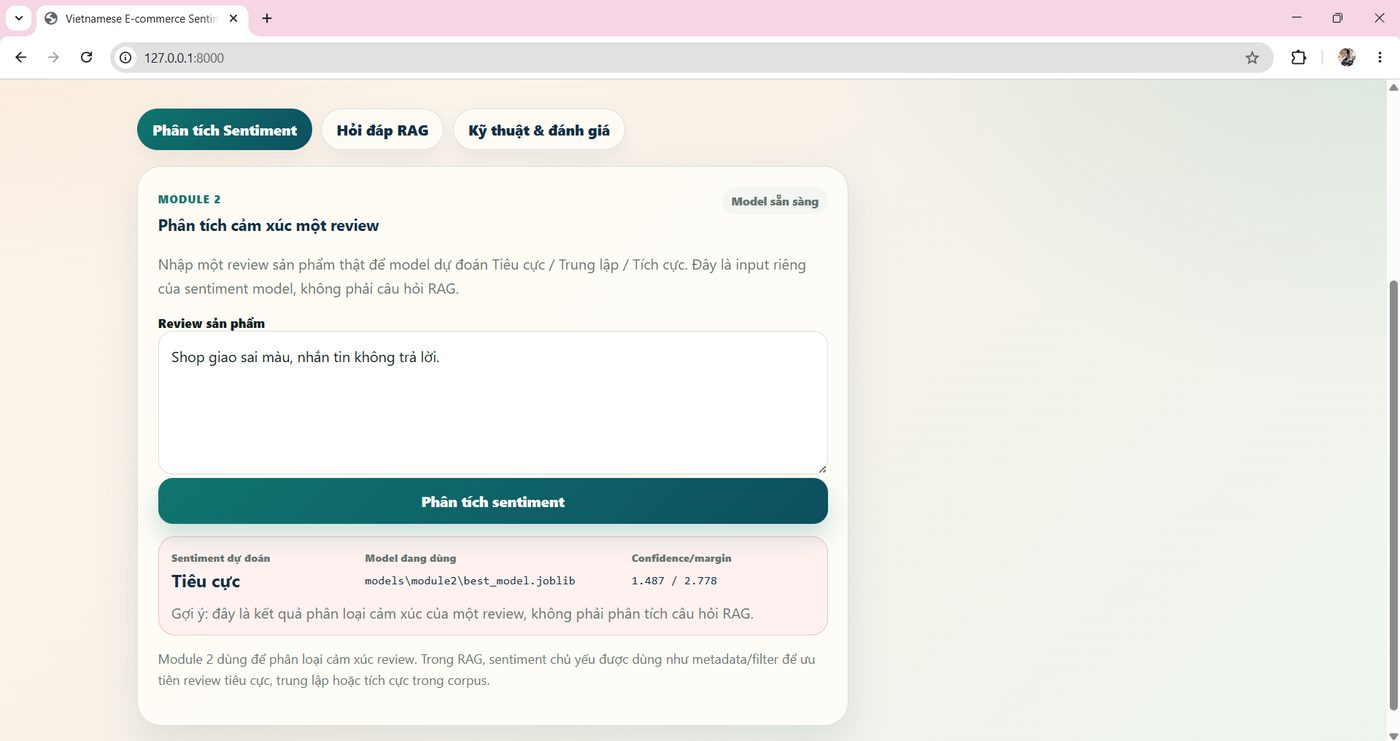
\includegraphics[width=0.92\textwidth]{figures_generated/web_sentiment_demo.jpg}
    \caption{Giao diện tab Phân tích Sentiment với ví dụ review tiêu cực.}
    \label{fig:web-sentiment-demo}
\end{figure}

Hình \ref{fig:web-rag-query-demo} thể hiện tab Hỏi đáp RAG ở bước nhập câu hỏi. Giao diện hiển thị các gợi ý truy vấn như giao hàng chậm, sai hàng, thiếu hàng, đóng gói lỗi hoặc chất lượng kém. Các gợi ý này giúp kiểm thử những nhóm complaint thường gặp trong review thương mại điện tử.

\begin{figure}[H]
    \centering
    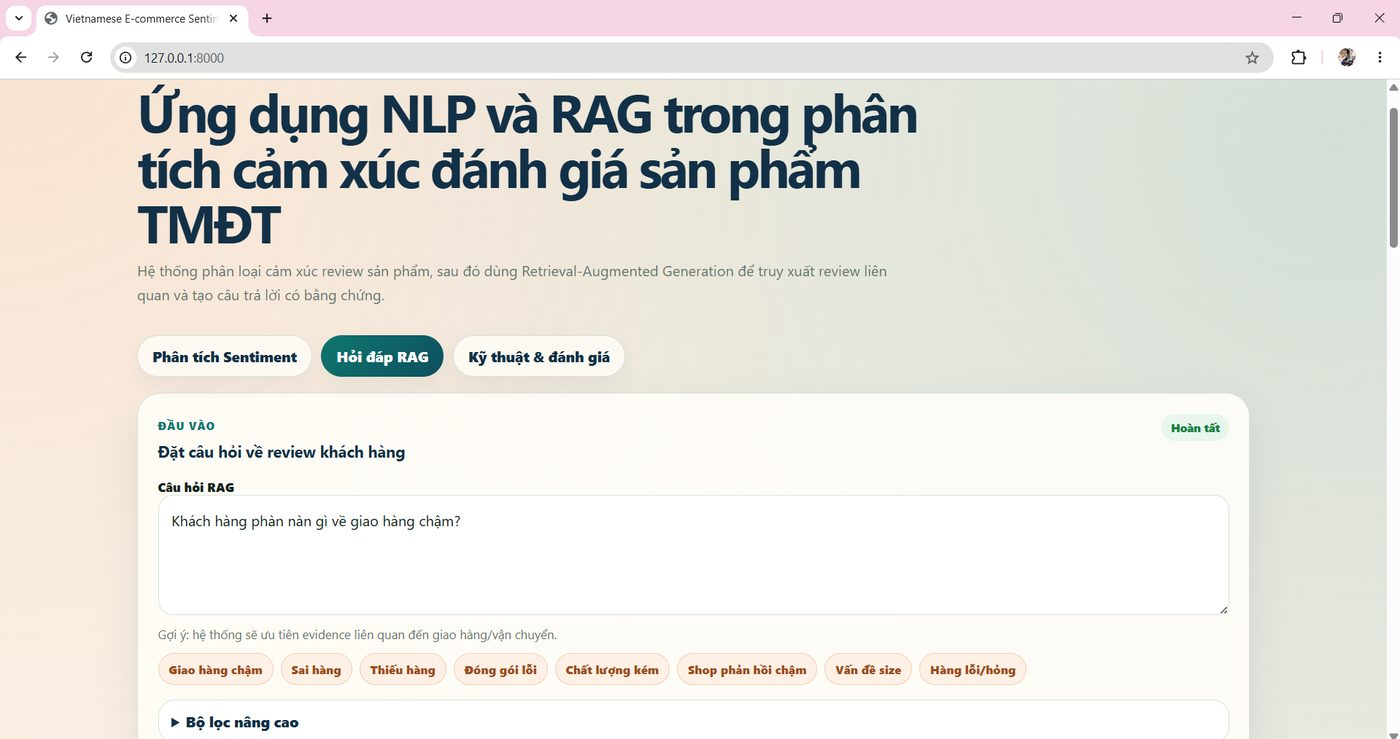
\includegraphics[width=0.92\textwidth]{figures_generated/web_rag_query_demo.jpg}
    \caption{Giao diện tab Hỏi đáp RAG ở bước nhập câu hỏi về review khách hàng.}
    \label{fig:web-rag-query-demo}
\end{figure}

\clearpage

Hình \ref{fig:web-rag-answer-demo} minh họa kết quả RAG sau khi thực thi truy vấn. Câu trả lời được trình bày theo hướng \EvidenceGrounded{}, gồm tóm tắt, các vấn đề chính, citation và danh sách evidence tiêu biểu. Cách trình bày này giúp người dùng không chỉ đọc kết luận tổng hợp mà còn kiểm tra được các review làm bằng chứng.

\begin{figure}[H]
    \centering
    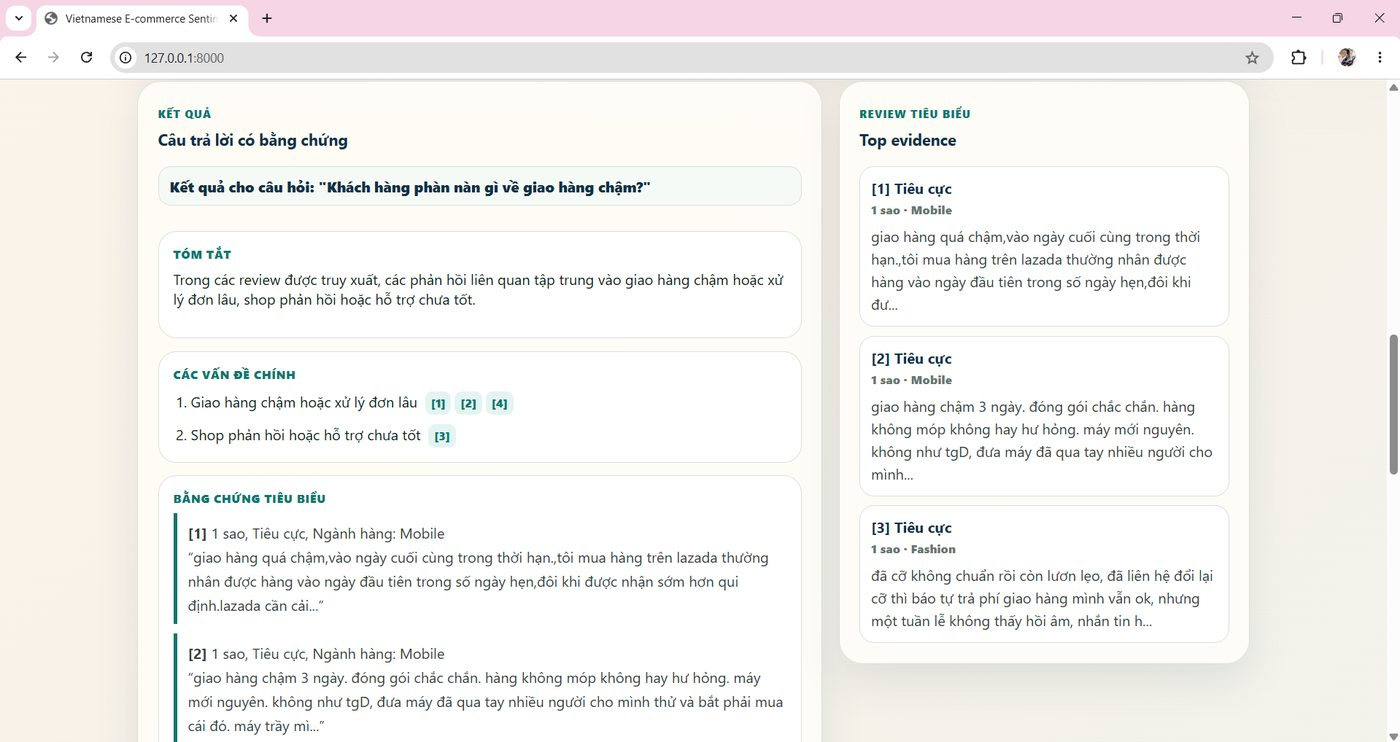
\includegraphics[width=0.92\textwidth]{figures_generated/web_rag_answer_demo.jpg}
    \caption{Kết quả RAG gồm tóm tắt, vấn đề chính, citation và top evidence.}
    \label{fig:web-rag-answer-demo}
\end{figure}

Hình \ref{fig:web-rag-evidence-demo} minh họa vùng review được truy xuất. Mỗi evidence card hiển thị citation id, điểm liên quan, ngành hàng, số sao, sentiment và đoạn review. Các từ khóa liên quan trong review được nhấn mạnh, giúp kiểm tra trực quan vì sao một review được xem là liên quan đến câu hỏi.

\begin{figure}[H]
    \centering
    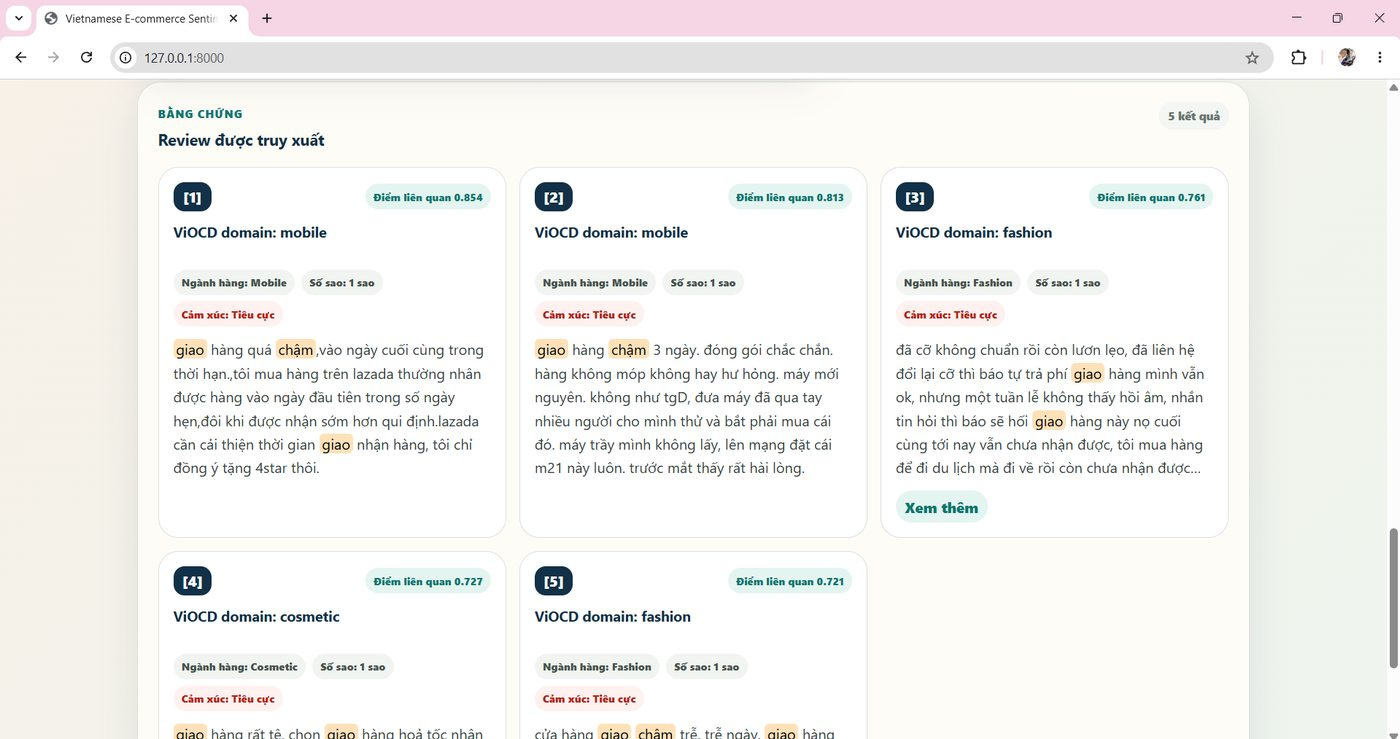
\includegraphics[width=0.92\textwidth]{figures_generated/web_rag_evidence_demo.jpg}
    \caption{Danh sách review được truy xuất trong tab RAG và các evidence cards.}
    \label{fig:web-rag-evidence-demo}
\end{figure}

Hình \ref{fig:web-technical-demo} minh họa tab Kỹ thuật \& đánh giá. Tab này tổng hợp các thông tin quan trọng của bản final như số documents trong kho review, embedding model, retrieval method và baseline Precision@5. Nhờ đó, người đọc có thể đối chiếu nhanh giữa giao diện demo và số liệu đã trình bày trong các chương dữ liệu, phương pháp và thực nghiệm.

\begin{figure}[H]
    \centering
    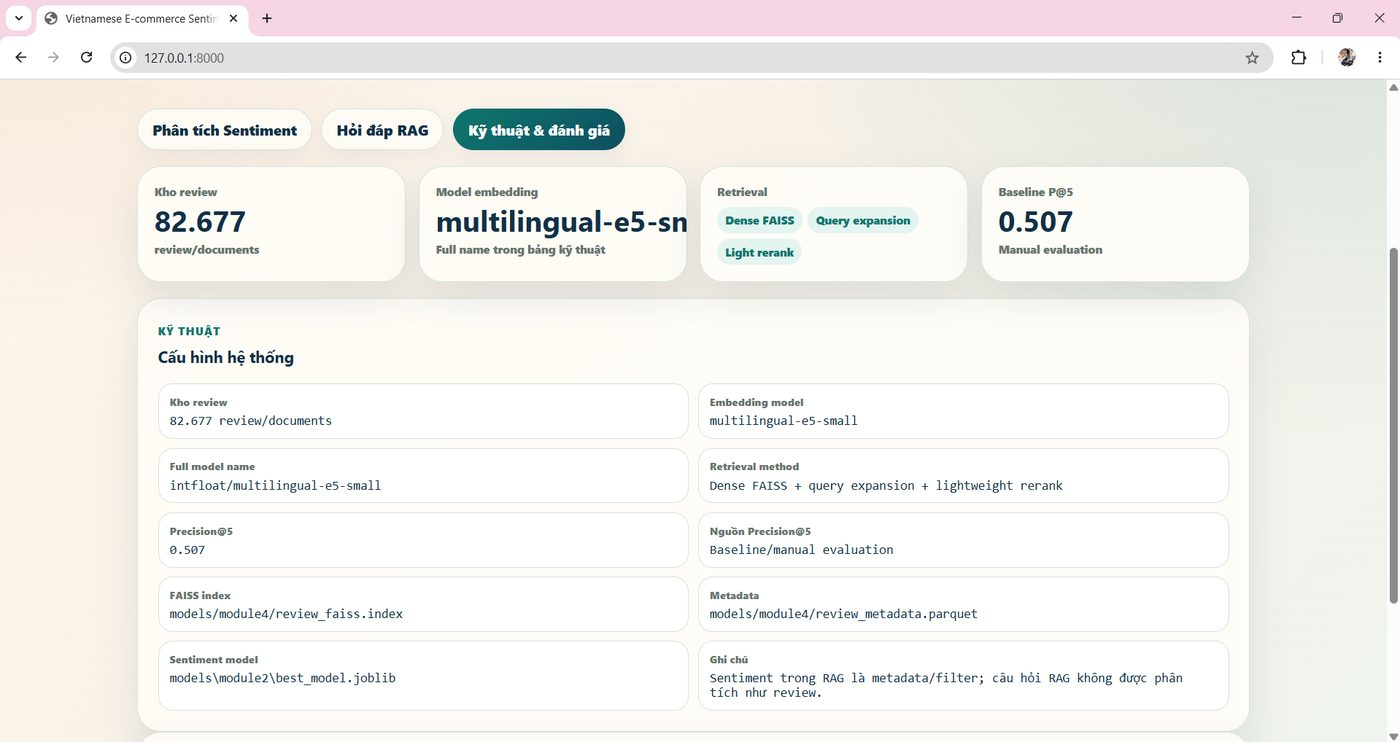
\includegraphics[width=0.92\textwidth]{figures_generated/web_technical_demo.jpg}
    \caption{Tab Kỹ thuật \& đánh giá hiển thị cấu hình hệ thống và metric chính.}
    \label{fig:web-technical-demo}
\end{figure}

\section{Vai trò của giao diện trong kiểm thử hệ thống}
Giao diện giúp kiểm thử tích hợp giữa các artifact và backend. Nếu tab Sentiment trả kết quả, có thể xác nhận artifact sentiment được load đúng. Nếu tab RAG trả answer có citation, có thể xác nhận FAISS index, metadata, embedding model và answer formatter hoạt động cùng nhau. Nếu tab kỹ thuật hiển thị 82.677 documents và embedding model multilingual-E5-small, có thể kiểm tra rằng cấu hình final của Module 4 đang được dùng.

Giao diện cũng hỗ trợ kiểm tra lỗi logic. Ví dụ, khi query thay đổi nhưng chưa chạy lại, UI cần cảnh báo để tránh hiển thị answer cũ như kết quả của query mới. Khi không có evidence đủ mạnh, answer phải trả lời thận trọng. Các kiểm soát này phản ánh nguyên tắc \EvidenceGrounded{} generation của đề tài.

\section{Tóm tắt triển khai}
Tầng triển khai thử nghiệm không làm thay đổi kết quả huấn luyện hoặc FAISS index. Nó đóng vai trò kết nối artifact đã có với người dùng thông qua API và UI. Vì vậy, nếu chỉ chỉnh giao diện hoặc format answer, không cần rebuild FAISS index. Nếu thay corpus, embedding model hoặc cách tạo retrieval text, cần build lại index/metadata và đánh giá lại retrieval.


\chapter{Thảo luận}
\section{\TFIDF{} + Linear SVM so với mô hình deep learning}
\TFIDF{} + Linear SVM là baseline cổ điển nhưng hiệu quả với text classification. Kết quả test \MacroFOne{} khoảng 0,9098 cho thấy với dữ liệu vừa, text ngắn và tín hiệu từ khóa rõ, mô hình tuyến tính vẫn mạnh. Ưu điểm là huấn luyện nhanh, dễ tái lập, ít tốn tài nguyên và dễ triển khai local.

So với PhoBERT hoặc XLM-R, \TFIDF{} + SVM không hiểu ngữ cảnh sâu, không tận dụng tốt ngữ nghĩa câu dài, phủ định phức tạp hoặc mỉa mai. Transformer có thể cải thiện nếu được fine-tune đủ tốt, nhưng cần GPU, thời gian và kiểm soát overfitting. Vì vậy trong project môn học, baseline cổ điển là lựa chọn hợp lý để có kết quả ổn định trước khi nâng cấp.

\section{Vai trò của RAG trong giải thích}
Sentiment model trả về nhãn, nhưng không tự trả lời được câu hỏi tổng hợp như “khách hàng phàn nàn gì về đóng gói”. RAG bổ sung khả năng truy xuất review liên quan và tạo insight có bằng chứng. Điều này làm hệ thống có tính giải thích hơn: không chỉ nói “tiêu cực”, mà chỉ ra review nào nói hộp móp, giao sai hoặc shop không trả lời.

RAG cũng giúp người dùng kiểm chứng. Nếu câu trả lời không hợp lý, người dùng có thể xem evidence card và biết hệ thống đã dựa vào review nào. Đây là điểm quan trọng trong bài toán review analytics.

\section{Sự khác nhau giữa sentiment prediction và RAG insight}
Sentiment prediction hoạt động ở mức một review. RAG insight hoạt động ở mức tập review được truy xuất theo query. Ví dụ, review “Hàng bị móp hộp” có thể được sentiment model phân loại negative. Nhưng query “Có vấn đề gì về đóng gói không?” cần tìm nhiều review liên quan, gom nhóm vấn đề và trả lời có citation. Hai phần này bổ trợ nhau nhưng không thay thế nhau.

\section{Ý nghĩa của Module 6}
Module 6 xuất phát từ hạn chế thực tế của dense retrieval. Các complaint ngắn thường phụ thuộc keyword chính xác. Hybrid retrieval cho phép kết hợp BM25 và dense FAISS, qua đó vừa giữ lexical precision vừa giữ semantic recall. Aspect-aware rules giúp hệ thống hiểu query theo khía cạnh như giao hàng, đóng gói, chất lượng, giá hoặc dịch vụ shop.

Tuy nhiên, Module 6 vẫn là MVP. Benchmark nhỏ cho thấy tín hiệu cải thiện keyword/aspect hit-rate, nhưng cần đánh giá relevance thủ công lớn hơn để kết luận chắc chắn.

\section{Bài học rút ra}
Bài học thứ nhất là dữ liệu quyết định rất nhiều đến chất lượng model. Nếu nhãn bị nhiễu hoặc duplicate không xử lý, metric sẽ thiếu tin cậy. Bài học thứ hai là retrieval cần đánh giá bằng relevance, không chỉ bằng score vector. Bài học thứ ba là giao diện phải phản ánh đúng logic hệ thống: sentiment và RAG cần tách input riêng. Bài học thứ tư là báo cáo nên trung thực về hạn chế, đặc biệt khi RAG chưa dùng LLM thật.


\chapter{Hạn chế và hướng phát triển}
\section{Hạn chế}
Hạn chế đầu tiên là nhãn sentiment được ánh xạ từ rating. Cách này nhanh và thực tế nhưng có thể nhiễu. Rating 3 sao không luôn là neutral; rating 5 sao vẫn có thể chứa phàn nàn; rating 1 sao có thể do yếu tố ngoài sản phẩm.

Hạn chế thứ hai là dataset sentiment chưa quá lớn. Với 5.162 review sau dedup, baseline có thể học tốt các từ khóa phổ biến nhưng chưa chắc tổng quát cho mọi ngành hàng. Lớp neutral ít hơn nên metric thấp hơn.

Hạn chế thứ ba là TF-IDF + SVM chưa hiểu ngữ cảnh sâu như PhoBERT/BERT. Mô hình có thể yếu với mỉa mai, phủ định phức tạp, câu dài nhiều ý và lỗi chính tả.

Hạn chế thứ tư là retrieval precision còn ở mức baseline. Manual Precision@5 khoảng 0,5067 cho thấy hệ thống đã truy xuất được evidence liên quan ở mức nhất định nhưng còn nhiều chỗ cải thiện. Top-k có thể lấy review cùng chủ đề nhưng sai intent hoặc sai polarity.

Hạn chế thứ năm là RAG chưa dùng LLM thật. Template-based generation an toàn và ổn định, nhưng khả năng diễn đạt và tổng hợp tự nhiên còn hạn chế. Nếu evidence phức tạp, template có thể chưa diễn giải tốt.

Hạn chế thứ sáu là Module 6 mới là MVP. Rule-based aspect sentiment chưa xử lý tốt phủ định, sarcasm, typo. Benchmark nhỏ chưa đủ để kết luận tổng quát.

\section{Hướng phát triển}
Hướng phát triển đầu tiên là fine-tune PhoBERT hoặc XLM-R cho sentiment classification. Điều này có thể cải thiện khả năng hiểu ngữ cảnh, đặc biệt với neutral/mixed sentiment.

Hướng thứ hai là xây dựng bộ dữ liệu ABSA tiếng Việt cho review TMĐT. Thay vì chỉ gán nhãn sentiment tổng thể, mỗi review có thể được gán aspect như chất lượng, giao hàng, đóng gói, dịch vụ shop và sentiment theo từng aspect.

Hướng thứ ba là huấn luyện supervised reranker cho retrieval. Reranker có thể học từ dữ liệu relevance thủ công để phân biệt review thật sự trả lời query và review chỉ cùng chủ đề.

Hướng thứ tư là mở rộng manual relevance evaluation. Bộ 15 query hiện tại quá nhỏ để kết luận mạnh. Cần nhiều query hơn, nhiều người chấm hơn và đo inter-annotator agreement.

Hướng thứ năm là tích hợp LLM có kiểm soát. Nếu dùng LLM, prompt phải bắt buộc dựa trên evidence, không được bịa, và câu trả lời phải có citation. LLM nên là lớp diễn đạt, không thay thế retrieval.

Hướng thứ sáu là cải thiện lọc spam/duplicate/noise. Có thể thêm model phát hiện review nhận xu, review không liên quan hoặc review copy-paste. Hướng thứ bảy là phát triển dashboard phân tích theo sản phẩm, category, thời gian và nhà bán.

\section{Định hướng production}
Nếu triển khai production, cần caching embedding/model, logging query, monitoring latency, kiểm soát version artifact, API authentication và cơ chế cập nhật index định kỳ. Hệ thống hiện tại mới là bản thử nghiệm học thuật end-to-end, chưa phải hệ thống production hoàn chỉnh.

\chapter{Kết luận}
Đề tài đã xây dựng được pipeline NLP/RAG end-to-end cho bài toán phân tích review TMĐT tiếng Việt. Phần sentiment classification xử lý dữ liệu, ánh xạ rating sang sentiment, chia train/valid/test và huấn luyện các baseline. Trong các mô hình đã thử, TF-IDF + Linear SVM đạt kết quả tốt nhất với test accuracy khoảng 0,9329 và test macro-F1 khoảng 0,9098.

Phần RAG xây dựng corpus/index final gồm 82.677 documents, dùng embedding model \code{intfloat/multilingual-e5-small}, FAISS \code{IndexFlatIP} và vector dim 384. Hệ thống truy xuất review liên quan theo query, áp dụng filter/rerank nhẹ và tạo câu trả lời template-based có citation. Manual Precision@5 baseline khoảng 0,5067 cho thấy retrieval đã hoạt động nhưng còn không gian cải thiện.

Đề tài cũng bổ sung Module 6 như hướng nâng cấp retrieval bằng BM25 + Dense FAISS + RRF/rerank + aspect rules. Benchmark nhỏ cho thấy hybrid retrieval cải thiện keyword/aspect hit-rate, nhưng cần đánh giá lớn hơn trước khi kết luận tổng quát. Giao diện thử nghiệm 3 tab giúp minh họa rõ sentiment, RAG và thông tin kỹ thuật.

Giá trị thực tiễn của đề tài là hỗ trợ tổng hợp phản hồi khách hàng TMĐT có bằng chứng. Thay vì chỉ đưa ra nhãn cảm xúc, hệ thống cho phép người dùng hỏi về vấn đề cụ thể và xem review thật làm nguồn. Báo cáo cũng chỉ ra hạn chế trung thực: nhãn sentiment có thể nhiễu, retrieval precision còn baseline, RAG chưa dùng LLM thật và Module 6 còn là MVP. Đây là nền tảng phù hợp để phát triển tiếp theo hướng transformer sentiment, supervised reranker, ABSA và LLM có kiểm soát.

\appendix
\chapter{Cấu trúc thư mục và artifact}

\section{Cấu trúc thư mục}
\begingroup
\small
\begin{longtable}{L{0.32\textwidth}L{0.58\textwidth}}
\caption{Cấu trúc thư mục chính của mã nguồn thực nghiệm}\label{tab:appendix-project-structure}\\
\toprule
Đường dẫn & Vai trò \\
\midrule
\filepath{backend/} & FastAPI backend cho API sentiment và RAG. \\
\filepath{frontend/} & HTML, CSS và JavaScript cho giao diện thử nghiệm. \\
\filepath{src/} & Mã nguồn xử lý dữ liệu, huấn luyện sentiment, retrieval/RAG và evaluation. \\
\filepath{scripts/} & Script chạy các module và web app. \\
\filepath{data/processed/} & Dữ liệu đã xử lý cho sentiment và RAG. \\
\filepath{data/reports/} & Summary dữ liệu và thống kê trung gian. \\
\filepath{data/eval/} & Query benchmark/evaluation. \\
\filepath{models/module2/} & Artifact của mô hình sentiment. \\
\filepath{models/module4/} & FAISS index và metadata RAG. \\
\filepath{results/module2..6/} & Metric, evaluation và output thử nghiệm. \\
\filepath{figures/module2..6/} & Hình minh họa dùng trong báo cáo. \\
\filepath{docs/} & Tài liệu kỹ thuật bổ sung. \\
\filepath{report_latex/} & Mã nguồn báo cáo LaTeX. \\
\bottomrule
\end{longtable}
\endgroup

\section{Artifact quan trọng}
\begingroup
\small
\begin{longtable}{L{0.24\textwidth}L{0.22\textwidth}L{0.16\textwidth}L{0.28\textwidth}}
\caption{Artifact chính và vai trò trong hệ thống}\label{tab:appendix-artifacts}\\
\toprule
Thư mục & Tên file & Nhóm & Vai trò \\
\midrule
\filepath{models/module2} & \code{best_model.joblib} & Sentiment & Model sentiment chính dùng khi inference. \\
\filepath{models/module2} & \code{tfidf_linearsvm.joblib} & Sentiment & Pipeline TF-IDF + Linear SVM, model tốt nhất trong baseline. \\
\filepath{models/module2} & \code{tfidf_logreg.joblib} & Sentiment & Pipeline TF-IDF + Logistic Regression để so sánh. \\
\filepath{models/module2} & \code{label_mapping.json} & Sentiment & Mapping nhãn negative/neutral/positive. \\
\filepath{models/module4} & \code{review_faiss.index} & Retrieval & Vector index FAISS cho 82.677 documents final. \\
\filepath{models/module4} & \code{review_metadata.parquet} & Retrieval & Metadata đồng bộ với từng vector trong FAISS. \\
\filepath{models/module4} & \code{module4_index_config.json} & Retrieval & Cấu hình embedding model, dim, index type, số documents và đường dẫn artifact. \\
\filepath{results/module2} & \code{metrics_summary.csv} & Evaluation & Metric train/valid/test của các mô hình sentiment. \\
\filepath{results/module5} & \code{manual_precision_overall.csv} & Evaluation & Manual Precision@3/5/10 của retrieval baseline. \\
\filepath{results/module6} & \code{last_benchmark_console_reference.txt} & Evaluation & Kết quả benchmark nhỏ của Module 6. \\
\bottomrule
\end{longtable}
\endgroup

\chapter{Hướng dẫn tái lập thực nghiệm}

\section{Môi trường}
Hệ thống được thiết kế để chạy local bằng Python. Các yêu cầu thư viện được chia theo từng phần nhằm giảm xung đột phụ thuộc:
\begin{itemize}
    \item \filepath{requirements_module1_2.txt}: xử lý dữ liệu và sentiment baseline.
    \item \filepath{requirements_module4.txt}: embedding, FAISS và retrieval/RAG.
    \item \filepath{requirements_module6.txt}: hybrid retrieval và benchmark mở rộng.
    \item \filepath{requirements_webapp.txt}: backend FastAPI và giao diện local.
\end{itemize}

\section{Thứ tự chạy}
Nếu cần tái lập từ đầu, thứ tự hợp lý là:
\begin{enumerate}
    \item Chạy Module 1 để tạo dữ liệu processed và summary.
    \item Chạy Module 2 để huấn luyện sentiment baseline và lưu model artifact.
    \item Chạy Module 3 để tạo thống kê/biểu đồ dữ liệu.
    \item Chạy Module 4 để chuẩn bị corpus, build FAISS index và đánh giá retrieval.
    \item Chạy Module 5 để tổng hợp metric, error analysis và report sections.
    \item Chạy Module 6 nếu cần đánh giá hướng hybrid retrieval.
    \item Chạy backend/frontend để kiểm tra inference tích hợp.
\end{enumerate}

\section{Lệnh chạy giao diện thử nghiệm}
\begin{lstlisting}[language=bash]
python -m pip install -r requirements_webapp.txt
python -m pip install -r requirements_module4.txt
python scripts/run_rag_webapp.py
\end{lstlisting}
Sau đó mở \code{http://127.0.0.1:8000}. Giao diện không yêu cầu API key vì answer generator là template-based.

\chapter{API backend}

\begingroup
\small
\begin{longtable}{L{0.20\textwidth}L{0.14\textwidth}L{0.30\textwidth}L{0.26\textwidth}}
\caption{Mô tả API backend}\label{tab:appendix-api}\\
\toprule
Endpoint & Method & Input & Output \\
\midrule
\code{/api/health} & GET & Không có & Trạng thái backend, corpus path, số review nếu load thành công. \\
\code{/api/config} & GET & Không có & Cấu hình model/index, danh sách category, metric hiển thị. \\
\code{/api/sentiment} & POST & \code{text}: nội dung review & Sentiment dự đoán và thông tin model. \\
\code{/api/rag} & POST & \code{query}, \code{top_k}, filter sentiment/category/rating & Answer có citation, evidence, query expansion và thông tin debug. \\
\bottomrule
\end{longtable}
\endgroup

\chapter{Ví dụ input/output}

\section{Sentiment classification}
Input:
\begin{lstlisting}[language=json]
{"text": "Shop giao sai mau, nhan tin ho tro nhung khong tra loi."}
\end{lstlisting}
Ví dụ trên tương ứng với review: “Shop giao sai màu, nhắn tin hỗ trợ nhưng không trả lời.”

Output rút gọn:
\begin{lstlisting}[language=json]
{
  "sentiment": "negative",
  "model": "TF-IDF + Linear SVM"
}
\end{lstlisting}

\section{RAG question answering}
Input:
\begin{lstlisting}[language=json]
{
  "query": "Khach hang phan nan gi ve giao hang cham?",
  "top_k": 5,
  "sentiment": "auto",
  "category": "all"
}
\end{lstlisting}
Ví dụ trên tương ứng với câu hỏi: “Khách hàng phàn nàn gì về giao hàng chậm?”

Output rút gọn:
\begin{lstlisting}[language=json]
{
  "summary": "Trong cac review duoc truy xuat, phan nan tap trung vao giao hang cham va ho tro sau ban chua tot.",
  "issues": [
    "Giao hang hoac xu ly don mat thoi gian.",
    "Mot so review phan anh giao sai hoac thieu hang."
  ],
  "evidence": [
    {"citation": 1, "rating": 1, "sentiment": "negative", "comment": "..."}
  ]
}
\end{lstlisting}

\chapter{Pseudocode pipeline}

\section{Huấn luyện sentiment}
\begin{keepcode}
\begin{lstlisting}[language=Python]
train, valid, test = load_sentiment_splits()
for params in tfidf_and_classifier_grid:
    model = train_pipeline(train.text, train.label, params)
    valid_pred = model.predict(valid.text)
    score = macro_f1(valid.label, valid_pred)
    keep_best_model(model, score)
test_pred = best_model.predict(test.text)
save_model(best_model)
save_metrics(test.label, test_pred)
\end{lstlisting}
\end{keepcode}

\section{Retrieval/RAG}
\begin{keepcode}
\begin{lstlisting}[language=Python]
query = clean_query(user_query)
expanded_query, filters = infer_query_intent(query)
query_embedding = e5_encode("query: " + expanded_query)
candidate_ids = faiss_search(query_embedding, candidate_k)
candidates = metadata.loc[candidate_ids]
candidates = apply_filters(candidates, filters)
evidence = rerank_and_select(candidates, top_k)
answer = template_answer(query, evidence, citations=True)
\end{lstlisting}
\end{keepcode}

\section{Module 6 hybrid retrieval}
\begin{keepcode}
\begin{lstlisting}[language=Python]
bm25_results = bm25_search(query, top_n)
dense_results = faiss_dense_search(query, top_n)
fused = reciprocal_rank_fusion([bm25_results, dense_results])
aspect = detect_aspect(query)
fused = apply_aspect_rules(fused, aspect)
final = rerank_or_fallback(query, fused)
return final.head(top_k)
\end{lstlisting}
\end{keepcode}

\chapter{Bảng metric bổ sung}

\section{Metric sentiment chính}
\begin{table}[H]
\centering
\caption{Tóm tắt metric sentiment chính trên tập test}
\label{tab:appendix-sentiment-metrics}
\begin{tabular}{lrrr}
\toprule
Mô hình & Accuracy & Macro-F1 & Weighted-F1 \\
\midrule
Majority baseline & 0,4297 & 0,2004 & 0,2583 \\
TF-IDF + Logistic Regression & 0,9174 & 0,8940 & 0,9176 \\
TF-IDF + Linear SVM & 0,9329 & 0,9098 & 0,9315 \\
\bottomrule
\end{tabular}
\end{table}

\section{Metric retrieval chính}
\begin{table}[H]
\centering
\caption{Manual Precision@k của retrieval baseline}
\label{tab:appendix-retrieval-metrics}
\begin{tabular}{lrrr}
\toprule
Metric & Giá trị & Số query & Số dòng đã gán nhãn \\
\midrule
Precision@3 & 0,4222 & 15 & 45 \\
Precision@5 & 0,5067 & 15 & 75 \\
Precision@10 & 0,4867 & 15 & 150 \\
\bottomrule
\end{tabular}
\end{table}

\section{Cấu hình RAG index final}
\begin{table}[H]
\centering
\caption[Cấu hình index RAG final]{Cấu hình index RAG final}
\label{tab:appendix-rag-config}
\begin{tabularx}{\textwidth}{L{0.32\textwidth}Y}
\toprule
Trường & Giá trị \\
\midrule
Số documents & 82.677 \\
Embedding model & \filepath{intfloat/multilingual-e5-small} \\
Embedding dim & 384 \\
Index type & FAISS \code{IndexFlatIP} \\
Similarity & Cosine via normalized inner product \\
Metadata & \code{review_metadata.parquet} \\
Index & \code{review_faiss.index} \\
\bottomrule
\end{tabularx}
\par\vspace{0.25em}
{\footnotesize Nguồn: \filepath{models/module4/module4_index_config.json}.}
\end{table}

\chapter{Ghi chú đạo đức và trách nhiệm}

Hệ thống xử lý review người dùng nên cần diễn giải kết quả thận trọng. Sentiment label trong đề tài được ánh xạ từ rating nên có thể nhiễu; không nên xem dự đoán sentiment là đánh giá tuyệt đối về khách hàng hoặc nhà bán. RAG answer chỉ phản ánh các review được truy xuất ở top-k, không đại diện cho toàn bộ thị trường nếu không có phân tích thống kê bổ sung.

Nếu triển khai ở môi trường thực tế, cần bổ sung cơ chế ẩn thông tin cá nhân, kiểm soát dữ liệu nhạy cảm, logging có giới hạn, versioning model/index và đánh giá human-in-the-loop. Các câu trả lời có citation giúp tăng tính minh bạch, nhưng vẫn cần người dùng kiểm tra evidence trước khi đưa ra quyết định vận hành.

\cleardoublepage
\addcontentsline{toc}{chapter}{Tài liệu tham khảo}
\begin{thebibliography}{99}

\bibitem{jurafsky2023speech}
D. Jurafsky and J. H. Martin.
\textit{Speech and Language Processing}.
Draft available online, 2023.

\bibitem{manning2008ir}
C. D. Manning, P. Raghavan, and H. Schütze.
\textit{Introduction to Information Retrieval}.
Cambridge University Press, 2008.

\bibitem{salton1988term}
G. Salton and C. Buckley.
Term-weighting approaches in automatic text retrieval.
\textit{Information Processing \& Management}, 24(5):513--523, 1988.

\bibitem{cortes1995support}
C. Cortes and V. Vapnik.
Support-vector networks.
\textit{Machine Learning}, 20:273--297, 1995.

\bibitem{fan2008liblinear}
R.-E. Fan, K.-W. Chang, C.-J. Hsieh, X.-R. Wang, and C.-J. Lin.
LIBLINEAR: A library for large linear classification.
\textit{Journal of Machine Learning Research}, 9:1871--1874, 2008.

\bibitem{pang2008opinion}
B. Pang and L. Lee.
Opinion mining and sentiment analysis.
\textit{Foundations and Trends in Information Retrieval}, 2(1--2):1--135, 2008.

\bibitem{liu2012sentiment}
B. Liu.
\textit{Sentiment Analysis and Opinion Mining}.
Morgan \& Claypool Publishers, 2012.

\bibitem{robertson2009probabilistic}
S. Robertson and H. Zaragoza.
The probabilistic relevance framework: BM25 and beyond.
\textit{Foundations and Trends in Information Retrieval}, 3(4):333--389, 2009.

\bibitem{cormack2009rrf}
G. V. Cormack, C. L. A. Clarke, and S. Büttcher.
Reciprocal rank fusion outperforms Condorcet and individual rank learning methods.
In \textit{Proceedings of SIGIR}, pages 758--759, 2009.

\bibitem{johnson2019billion}
J. Johnson, M. Douze, and H. Jégou.
Billion-scale similarity search with GPUs.
\textit{IEEE Transactions on Big Data}, 7(3):535--547, 2019.

\bibitem{lewis2020rag}
P. Lewis, E. Perez, A. Piktus, F. Petroni, V. Karpukhin, and others.
Retrieval-Augmented Generation for Knowledge-Intensive NLP Tasks.
In \textit{Advances in Neural Information Processing Systems}, 2020.

\bibitem{devlin2019bert}
J. Devlin, M.-W. Chang, K. Lee, and K. Toutanova.
BERT: Pre-training of Deep Bidirectional Transformers for Language Understanding.
In \textit{Proceedings of NAACL-HLT}, 2019.

\bibitem{conneau2020xlmr}
A. Conneau, K. Khandelwal, N. Goyal, and others.
Unsupervised Cross-lingual Representation Learning at Scale.
In \textit{Proceedings of ACL}, 2020.

\bibitem{nguyen2020phobert}
D. Q. Nguyen and A. T. Nguyen.
PhoBERT: Pre-trained language models for Vietnamese.
In \textit{Findings of EMNLP}, pages 1037--1042, 2020.

\bibitem{reimers2019sentencebert}
N. Reimers and I. Gurevych.
Sentence-BERT: Sentence Embeddings using Siamese BERT-Networks.
In \textit{Proceedings of EMNLP-IJCNLP}, 2019.

\bibitem{wang2022e5}
L. Wang, N. Yang, X. Huang, B. Jiao, L. Yang, D. Jiang, R. Majumder, and F. Wei.
Text Embeddings by Weakly-Supervised Contrastive Pre-training.
\textit{arXiv preprint arXiv:2212.03533}, 2022.

\bibitem{nogueira2019passage}
R. Nogueira and K. Cho.
Passage Re-ranking with BERT.
\textit{arXiv preprint arXiv:1901.04085}, 2019.

\bibitem{vaswani2017attention}
A. Vaswani, N. Shazeer, N. Parmar, and others.
Attention Is All You Need.
In \textit{Advances in Neural Information Processing Systems}, 2017.

\bibitem{pedregosa2011scikit}
F. Pedregosa, G. Varoquaux, A. Gramfort, and others.
Scikit-learn: Machine Learning in Python.
\textit{Journal of Machine Learning Research}, 12:2825--2830, 2011.

\bibitem{khattab2020colbert}
O. Khattab and M. Zaharia.
ColBERT: Efficient and Effective Passage Search via Contextualized Late Interaction over BERT.
In \textit{Proceedings of SIGIR}, 2020.

\bibitem{karpukhin2020dense}
V. Karpukhin, B. Oğuz, S. Min, P. Lewis, L. Wu, S. Edunov, D. Chen, and W.-t. Yih.
Dense Passage Retrieval for Open-Domain Question Answering.
In \textit{Proceedings of EMNLP}, 2020.

\bibitem{pontiki2014semeval}
M. Pontiki, D. Galanis, J. Pavlopoulos, H. Papageorgiou, I. Androutsopoulos, and S. Manandhar.
SemEval-2014 Task 4: Aspect Based Sentiment Analysis.
In \textit{Proceedings of the 8th International Workshop on Semantic Evaluation}, 2014.

\bibitem{fastapi}
S. Ramirez.
FastAPI Documentation.
\url{https://fastapi.tiangolo.com/}, 2018.

\end{thebibliography}


\end{document}

